\chapter{Εντοπισμός Σημείων Αλλαγής της Χρονοσειράς \tl{B}}
\label{ch:step5}
\thispagestyle{fancy}

Παιρνώντας στο βήμα 5, θα επαναλάβουμε τη διαδικασία και ανάλυση του βήματος 4 στη χρονοσειρά προβολών του βίντεο \tl{B}, για την οποία επίσης θα γίνει προσπάθεια ανίχνευσης σημείων σημαντικών αλλαγών με αυτόματο τρόπο.

\par Η μέθοδος και το κριτήριο επιλογής των σημείων αλλαγής παραμένουν τα ίδια με το προηγούμενο βήμα όπως επίσης και οι επιλογές αναπροσαρμογής του μοντέλου κατά τη διάρκεια εφαρμογής της μεθόδου. Επίσης και εδώ έχουν υλοποιηθεί και οι τρεις επιλογές.

\section{Αρχική Εφαρμογή}

Αρχικά, θα δώσουμε κάποιες τιμές στις \tl{hyperparameters} της μεθόδου, δηλαδή στο μέγεθος εκπαίδευσης $n_0$, στον ορίζοντα πρόβλεψης, $T$, στην επιλογή αναπροσαρμογής του μοντέλου και στην παράμετρο $\lambda_{std}$, και θα τρέξουμε την παραπάνω μέθοδο στη στάσιμη χρονοσειρά που προέκυψε από το βήμα \ref{ch:step3}, $\{X_{b_{deseasoned}}(t)\}$, και στο $ARMA(4,4)$ μοντέλο που προσαρμόστηκε σε αυτή (σχέση \ref{eq:xb_deseasoned_4_4_model}). Έτσι, για τις παραμέτρους θα έχουμε:
\renewcommand{\labelitemi}{\textendash}
\begin{itemize}
    \item $n_0=400$: Όπως προτείνεται στην εκφώνηση, το μέγεθος εκπαίδευσης θα είναι 400 παρατηρήσεις
    \item $T=5$: Επίσης δίνεται έμμεσα στην εκφώνηση, το κριτήριο αρχικά θα υπολίζεται για προβλέψεις έως και 5 βήματα εμπρός
    \item $choice="c"$: Διατήρηση του μοντέλου έως ότου βρεθεί σημείο αλλαγής και επαναπροσαρμογή του στις 400 πιο πρόσφατες παρατηρήσεις από το $n+5$ όταν βρεθεί
    \item $\lambda_{std}=\sqrt{2}$: Όχι σε συμφωνία με την προτεινόμενη τιμή, καθώς αυτή δίνει μόλις ένα σημειο αλλαγής για τις υπόλοιπες επιλεγμένες παραμέτρους, αλλά ως μία τυχαία αρχική επιλογή. Άρα, κριτήριο επλογής \tl{MCPs} όταν $S_n > \sqrt{2} * s_x$
\end{itemize}

\par Παρακάτω, φαίνονται τα σημεία αλλαγής που προκύπτουν από την εκτέλεση της μεθόδους με τις παραπάνω παραμέτρους:

\begin{figure}[H]
    \begin{center}
        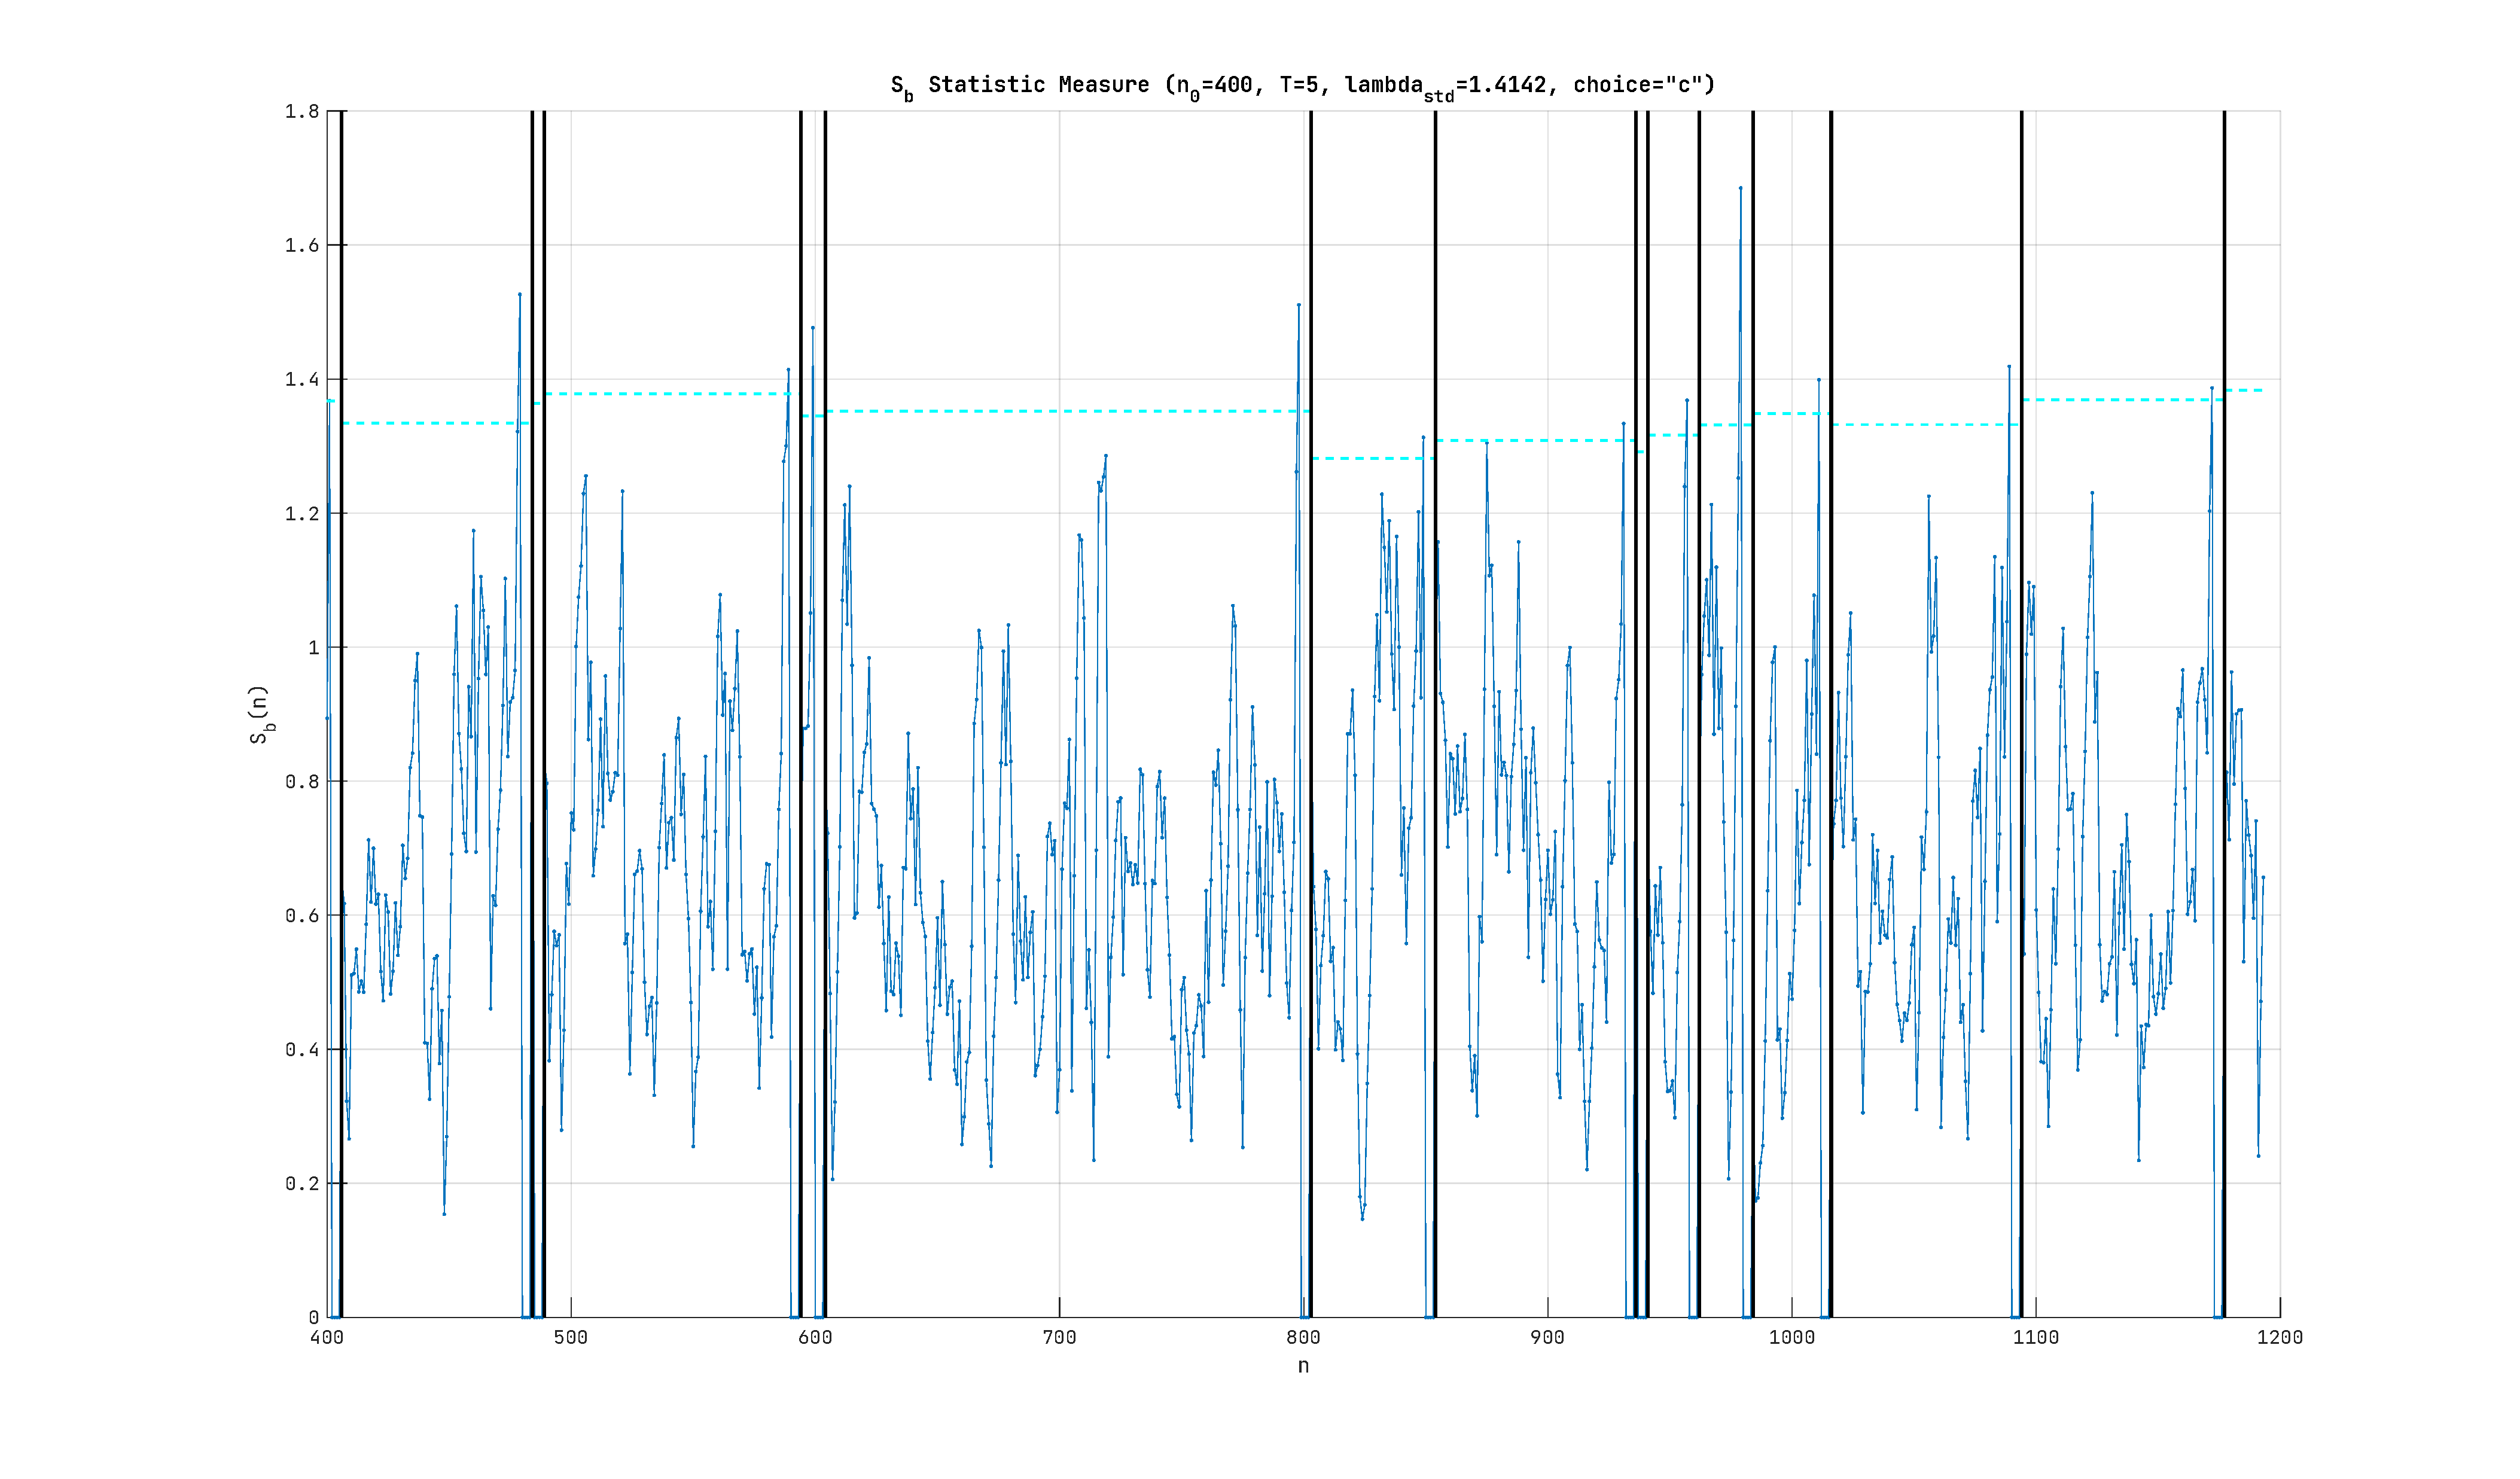
\includegraphics[width=\textwidth]{plots/mcps_xb.svg.pdf}
        \caption{Τιμές στατιστικού $S_n$ για έως και 5 βήματα μπροστά πρόβλεψη με $ARMA(4,4)$ της στάσιμης χρονοσειράς $\{X_{b_{deseasoned}}(t)\}$. Σημειώνονται επίσης το κριτήριο απόφασης, $\alpha$, (\tl{cyan}) και φυσικά τα σημεία αλλαγής με έντονες κάθετες γραμμές στα εκάστοτε σημεία $n+T$ (μαύρο). Το $n$ ξεκινάει από το 400 και άρα το $S_n$ δεν ορίζεται για τιμές $n<n_0=400$.}
        \label{fig:mcps_xb}
    \end{center}
\end{figure}

Όπως φαίνεται στο παραπάνω διάγραμμα, επειδή έχει χρησιμοποιηθεί η επιλογή \textquote{\tl{c}} για την αναπροσαρμογή του μοντέλου, κάθε φορά που εντοπίζεται σημείο αλλαγής το μοντέλο επανεκτιμάται σε νέο \tl{training set} (που είναι οι τελευταίες 400 παρατηρήσεις από τη στιγμή $n+5$) και άρα αλλάζει η δειγματική τυπική απόκλιση των παρατηρήσεων του \tl{training set}. Αυτό φαίνεται ως αλλαγή στο επίπεδο της \tl{cyan} διακεκομμένης γραμμής μεταξύ διαδοχικών σημειών αλλαγής. 

\par Παρακάτω, τα ίδια σημεία αλλαγής απεικονίζονται στην αρχική χρονοσειρά προβολών του βίντεο \tl{B} και κατόπιν ακολουθεί σύντομος σχολιασμός:

\begin{figure}[H]
    \begin{center}
        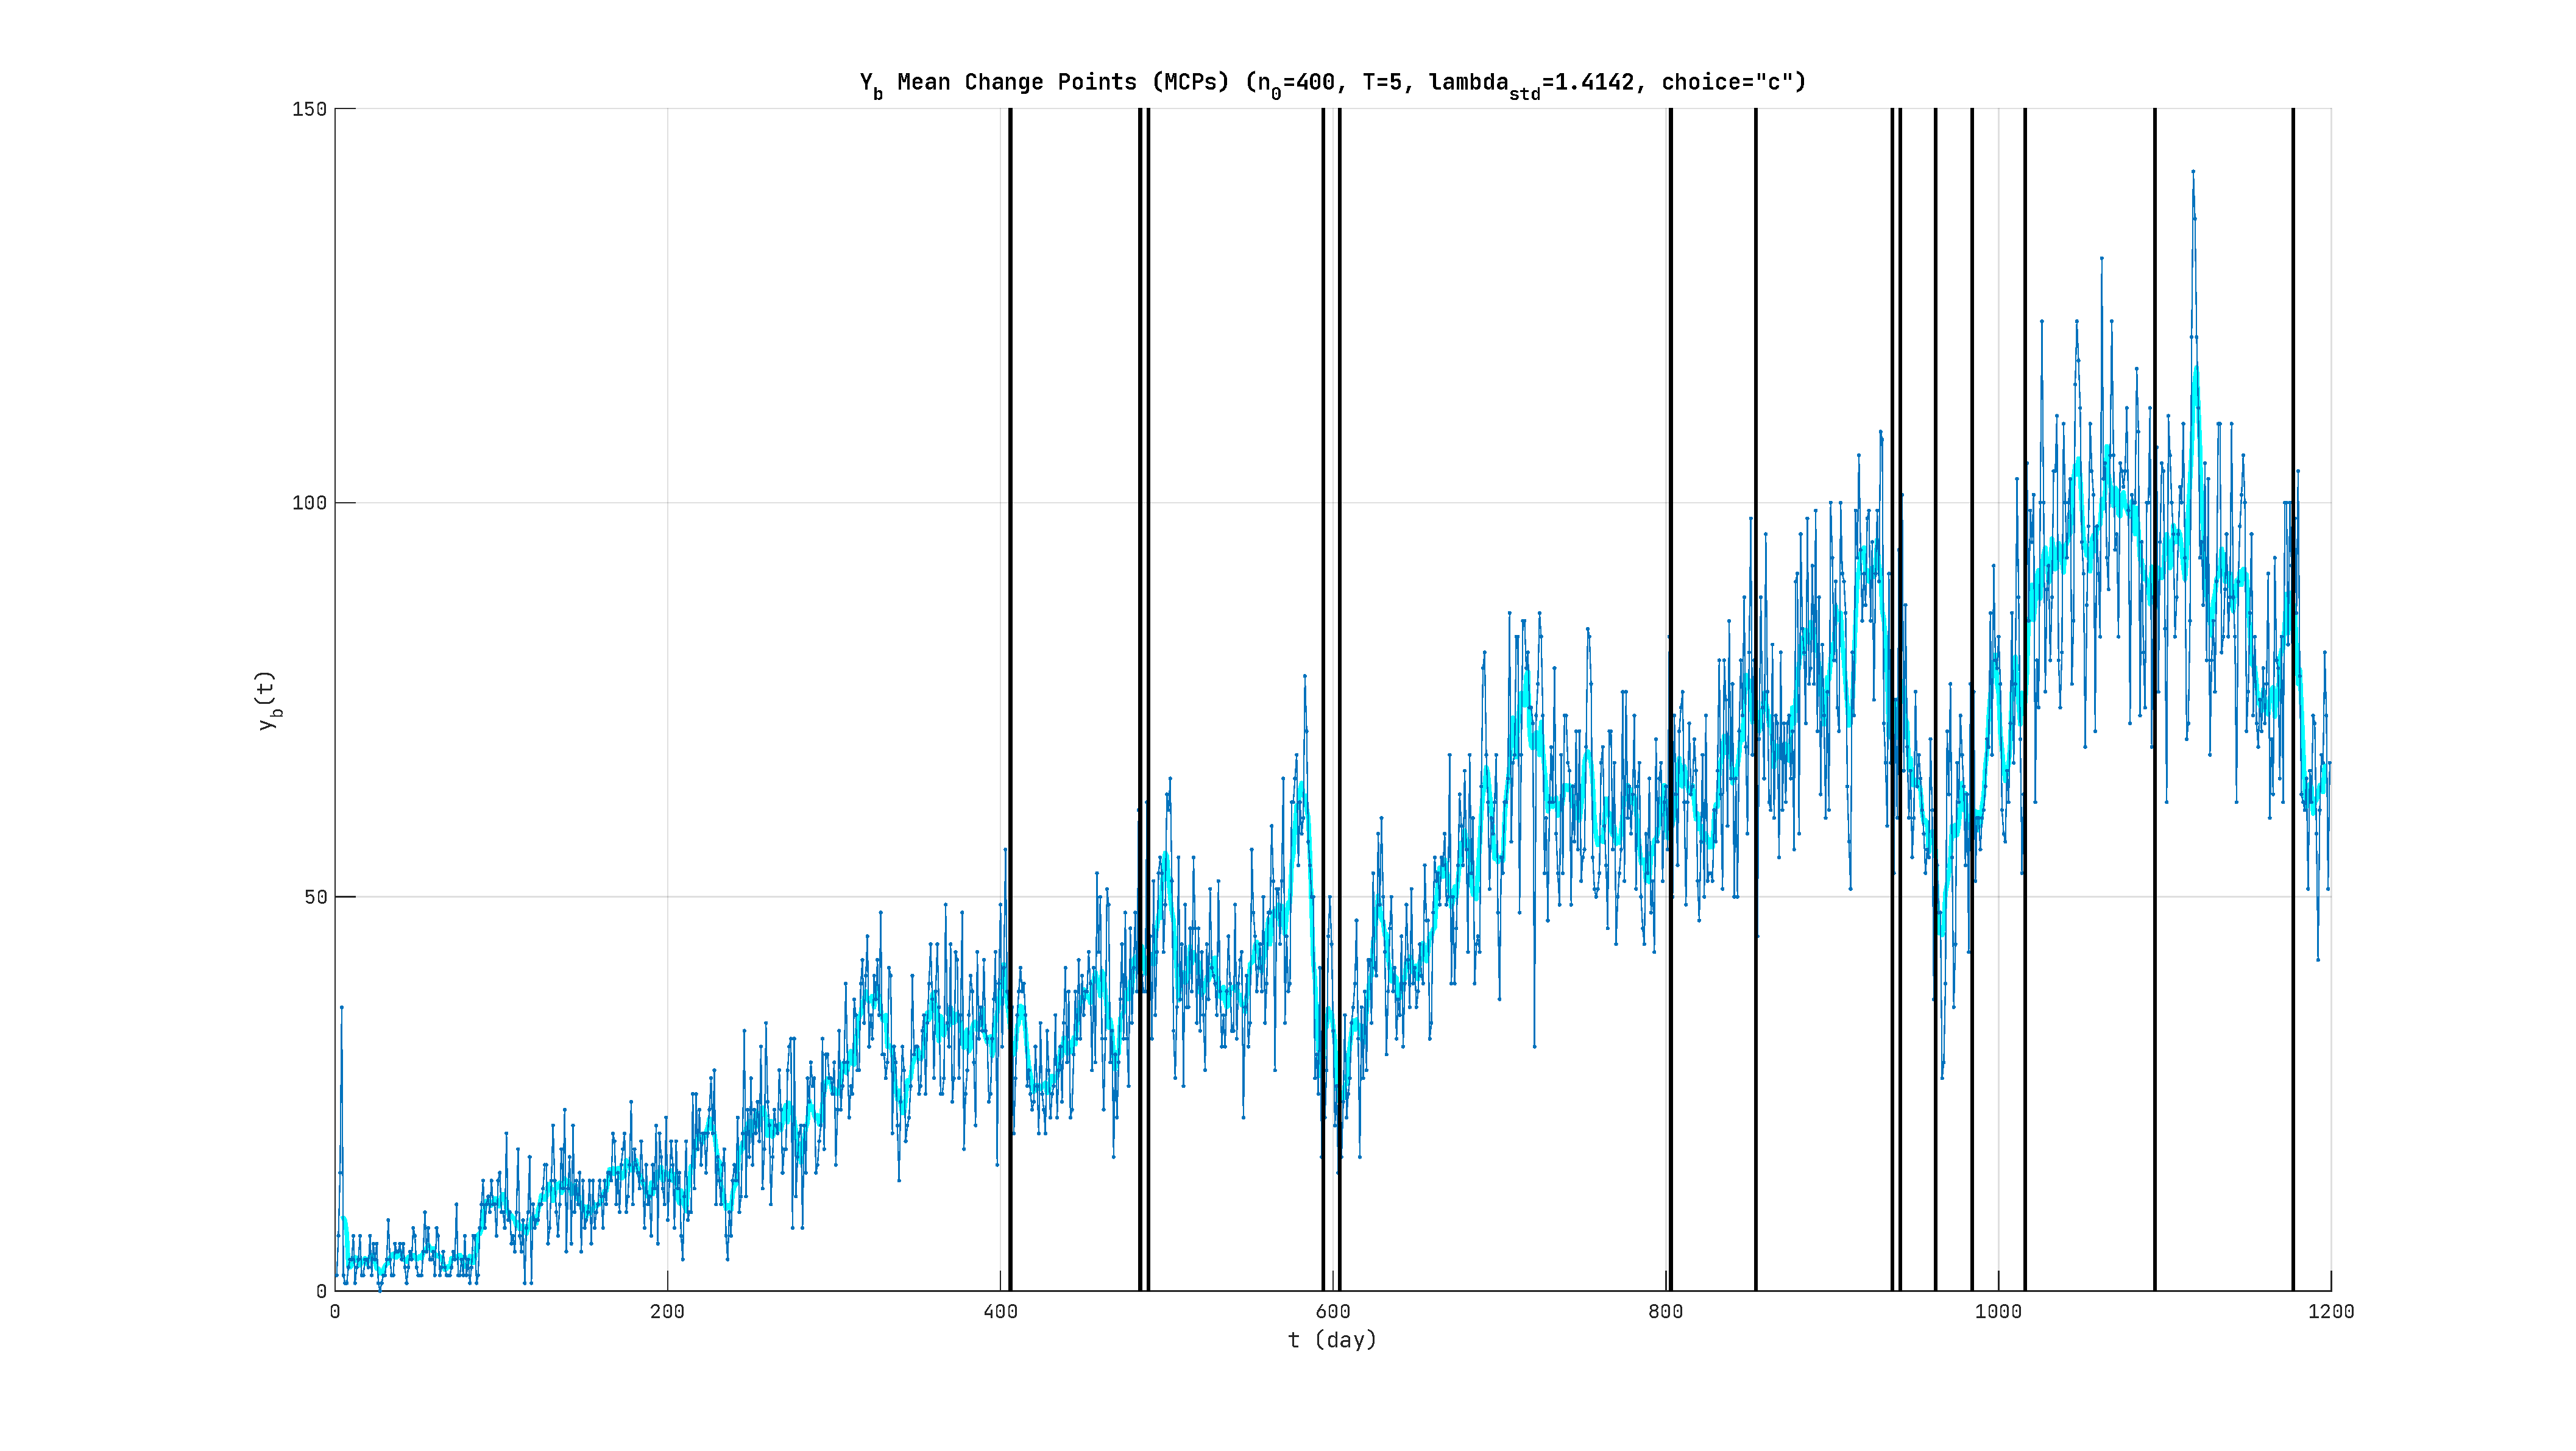
\includegraphics[width=\textwidth]{plots/mcps_yb.svg.pdf}
        \caption{Διάγραμμα ιστορίας της αρχικής χρονοσειράς $\{Y_b(t)\}$ (μπλε) μαζί με τα σημεία αλλαγής (μαύρο) που επιλέχθηκαν από την ανάλυση της στάσιμης εκδοχής της, καθώς και εκτίμηση της τάσης με φίλτρο κινούμενου μέσου τάξης 7 ($MA(7)$ \tl{smoothing})}
        \label{fig:mcps_yb}
    \end{center}
\end{figure}

Βλέποντας το πού \textquote{πέφτουν} τα 14 σημεία αλλαγής στην αρχική χρονοσειρά προβολών του βιντέο \tl{B} παρατηρούμε πως αυτά δεν είναι σε τυχαίες θέσεις. Βρίσκοντα και εδώ (όπως και στην ανάλυση της πρώτης χρονοσειράς) είτε σε κορυφές, δηλαδή σε θέσεις που αριστερά υπάρχει τοπικά αυξητική τάση και δεξιά τοπικά πτωτική (ακόμα και εάν αυτό γίνεται για λίγες παρατηρήσεις), ή σε βυθούς, δηλαδή σε σημεία που αριστερά υπάρχει τοπικά πτωτική τάση ενώ δεξία αυτή αλλάζει και γίνεται αυξυτική. Είναι κάπως λογικό οι προβλέψεις μας για τις γειτονιές τέτοιων σημείων (ακόμα και εάν γίνονται μέσω στάσιμων εκδοχών των αρχικών χρονοσειρών) με γραμμικά μοντέλα να εμφανίζουν αρκετά σημαντικά σφάλματα ώστε να σηματοδοτηθούν σημεία αλλαγής.

\par Ακολουθεί μια πιο ενδελεχής ανάλυση για την επιλογή των \tl{hyperparameters} που σε αυτήν την υποενότητα έγινε κάπως αυθαίρετα.

\section{Επιλογή Βέλτιστων \tl{Hyperparameters}}

Για επιλογή βέλτιστων τιμών στις \tl{hyperparameters} της μεθόδου και συγκεκριμένα στον ορίζοντα πρόβλεψης, $T$, και στο $\lambda_{std}$ του ορίου απόφασης, $\alpha$, θα κάνουμε αναζήτηση πλέγματος ως προς αυτές. Ως μετρικές για αξιολόγηση του κάθε συνδυασμού των παραμέτρων αυτών χρησιμοποιήθηκαν οι ίδιες όπως και στη ανάλυση πρώτης χρονοσειράς, δηλαδή ο \textit{Αριθμός \tl{MCPs}} και το \textit{\tl{NRMSE} Προβλέψεων}.

Αρχικά παραθέτονται σε διαγράμματα τύπου \tl{surf} τα αποτελέσματα αναζήτησης πλέγματος ως προς τις παραπάνω μετρικές ενώ στη συνέχεια σχολιάζεται ο τρόπος επιλογής προσεγγεστικά βέλτιστων παραμάτρων αλλά και οι τελικές τους τιμές.

\begin{figure}[H]
    \begin{center}
        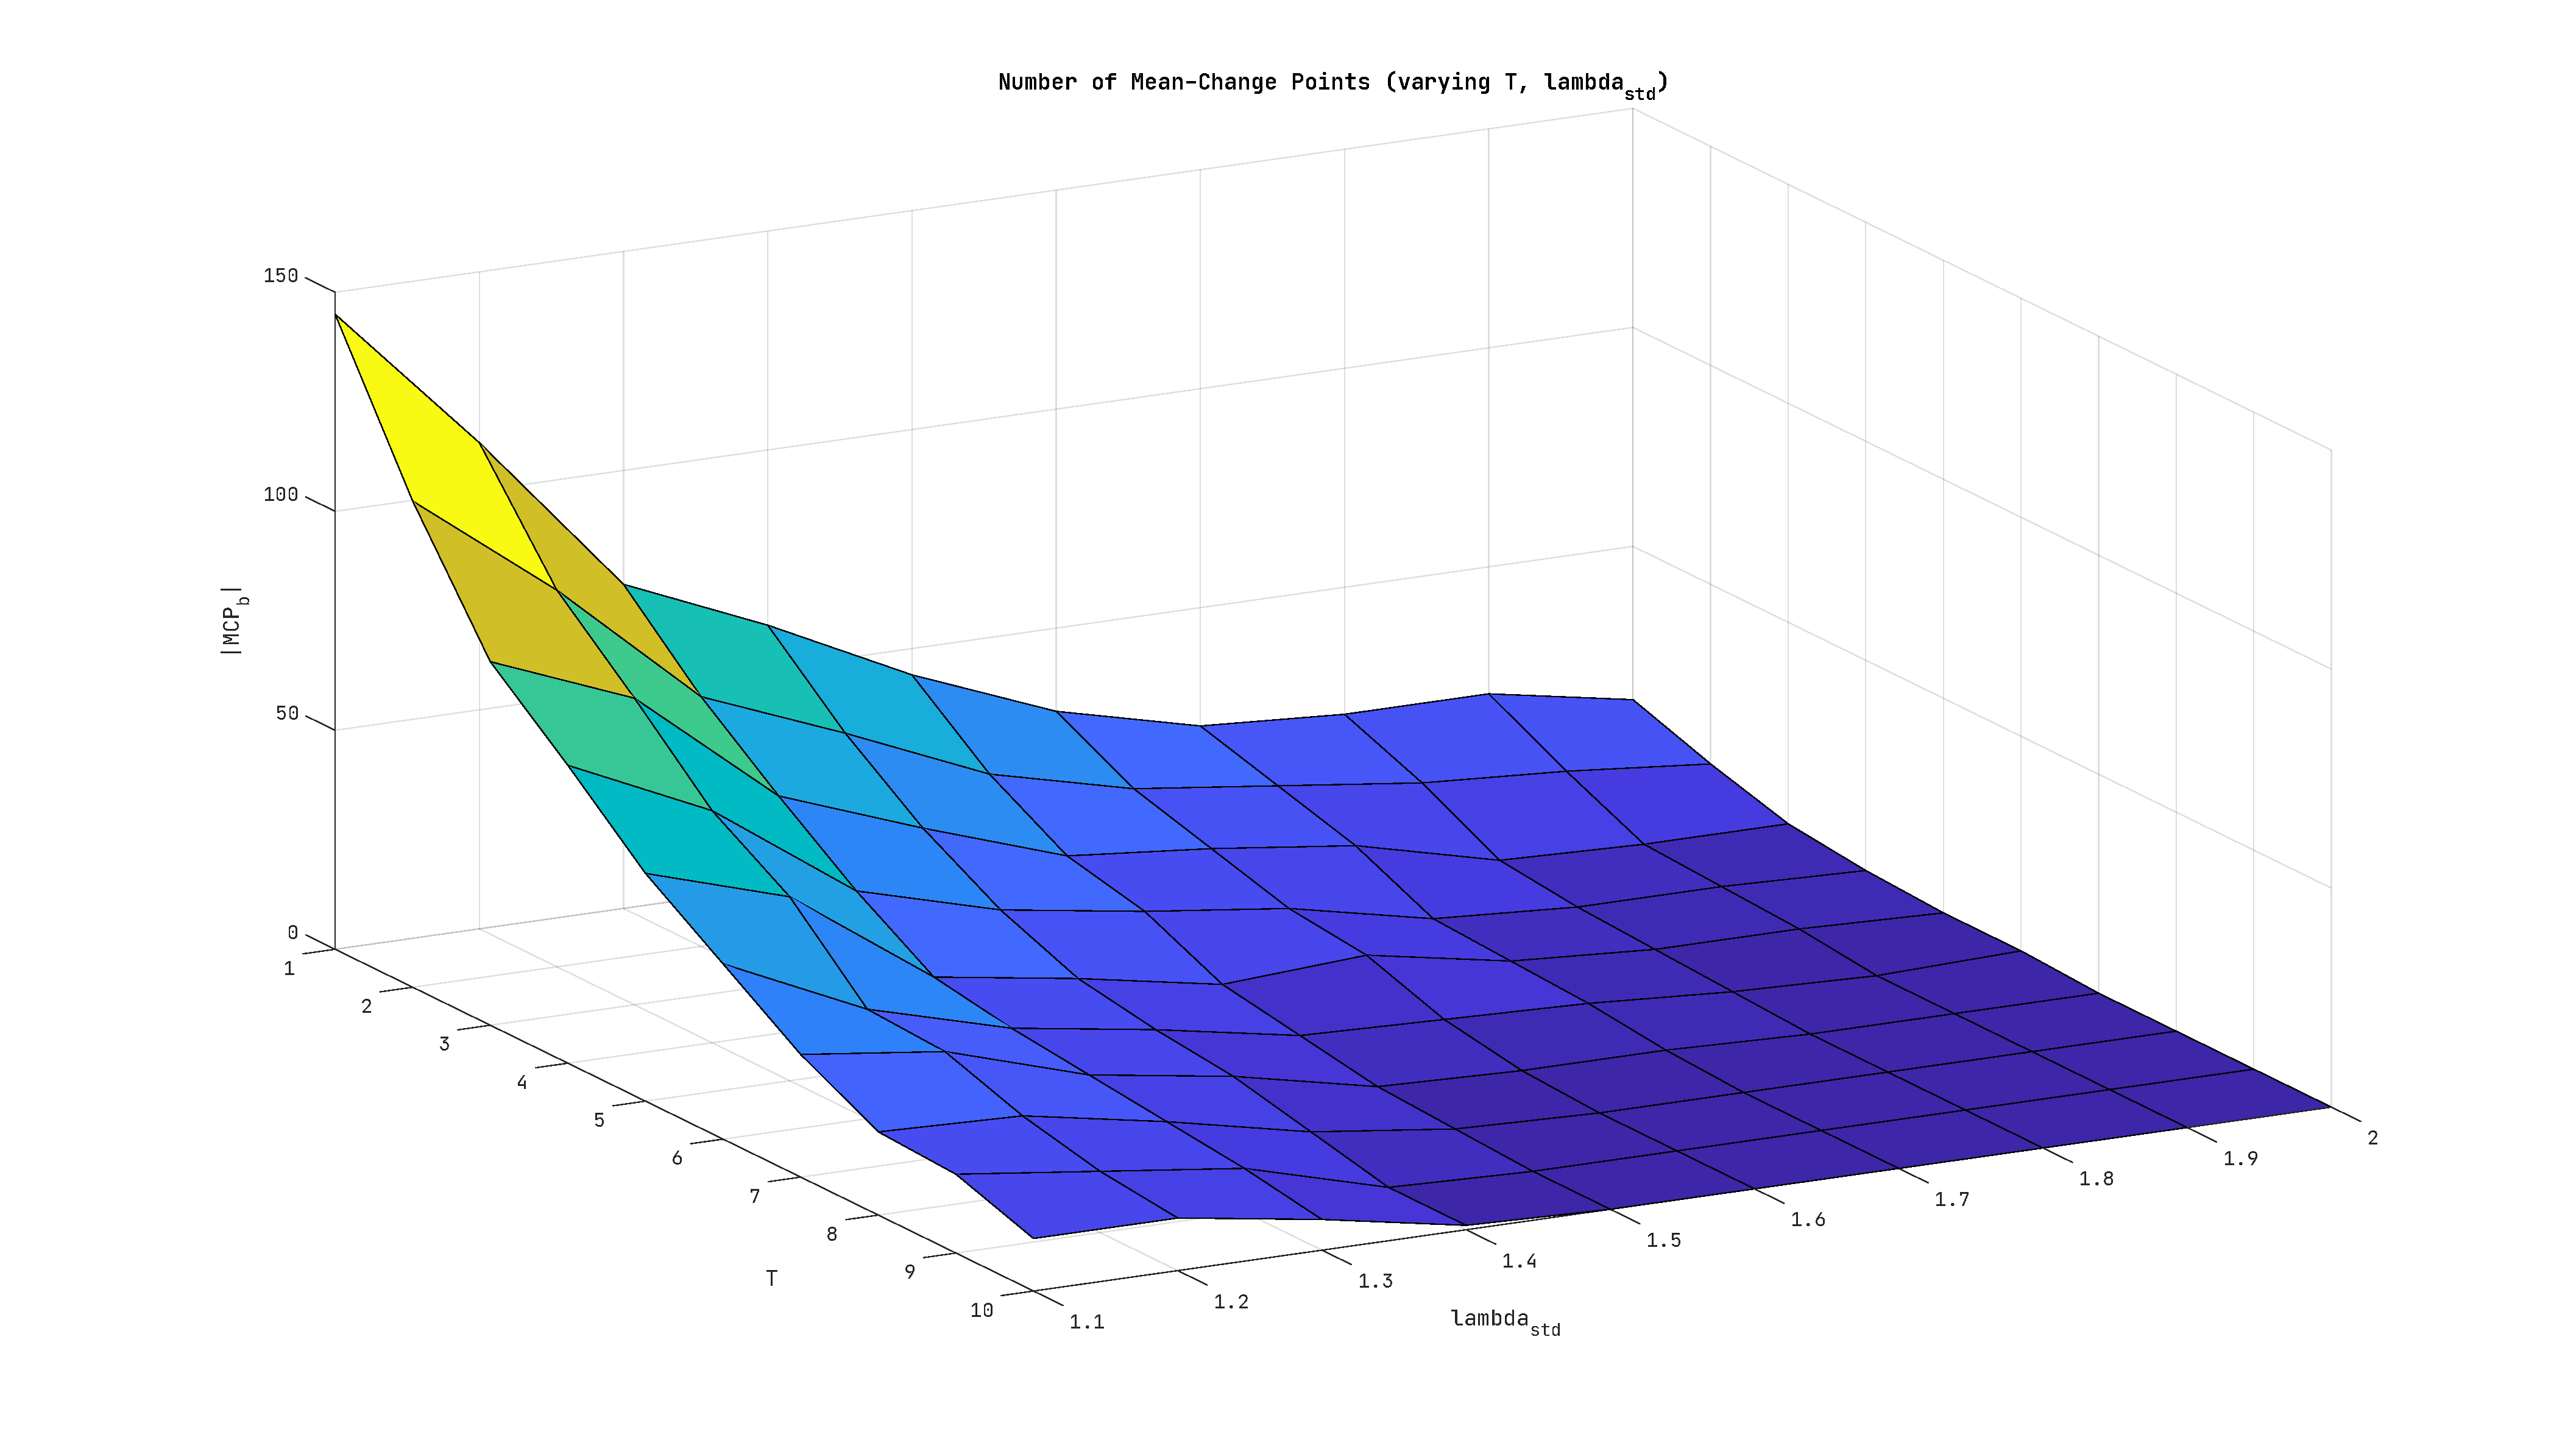
\includegraphics[width=\textwidth]{plots/mcps_count_b.svg.pdf}
        \caption{Αριθμός σημείων αλλαγής, $\vert$\tl{MCP}$\vert$, που προκύπτουν για κάθε τιμή του πλέγματος αναζήτησης ως πρός τον ορίζοντα πρόβλεψης, $T$, και το $\lambda_{std}$ του ορίου απόφασης, $\alpha$}
        \label{fig:mcps_count_b}
    \end{center}
\end{figure}

\begin{figure}[H]
    \begin{center}
        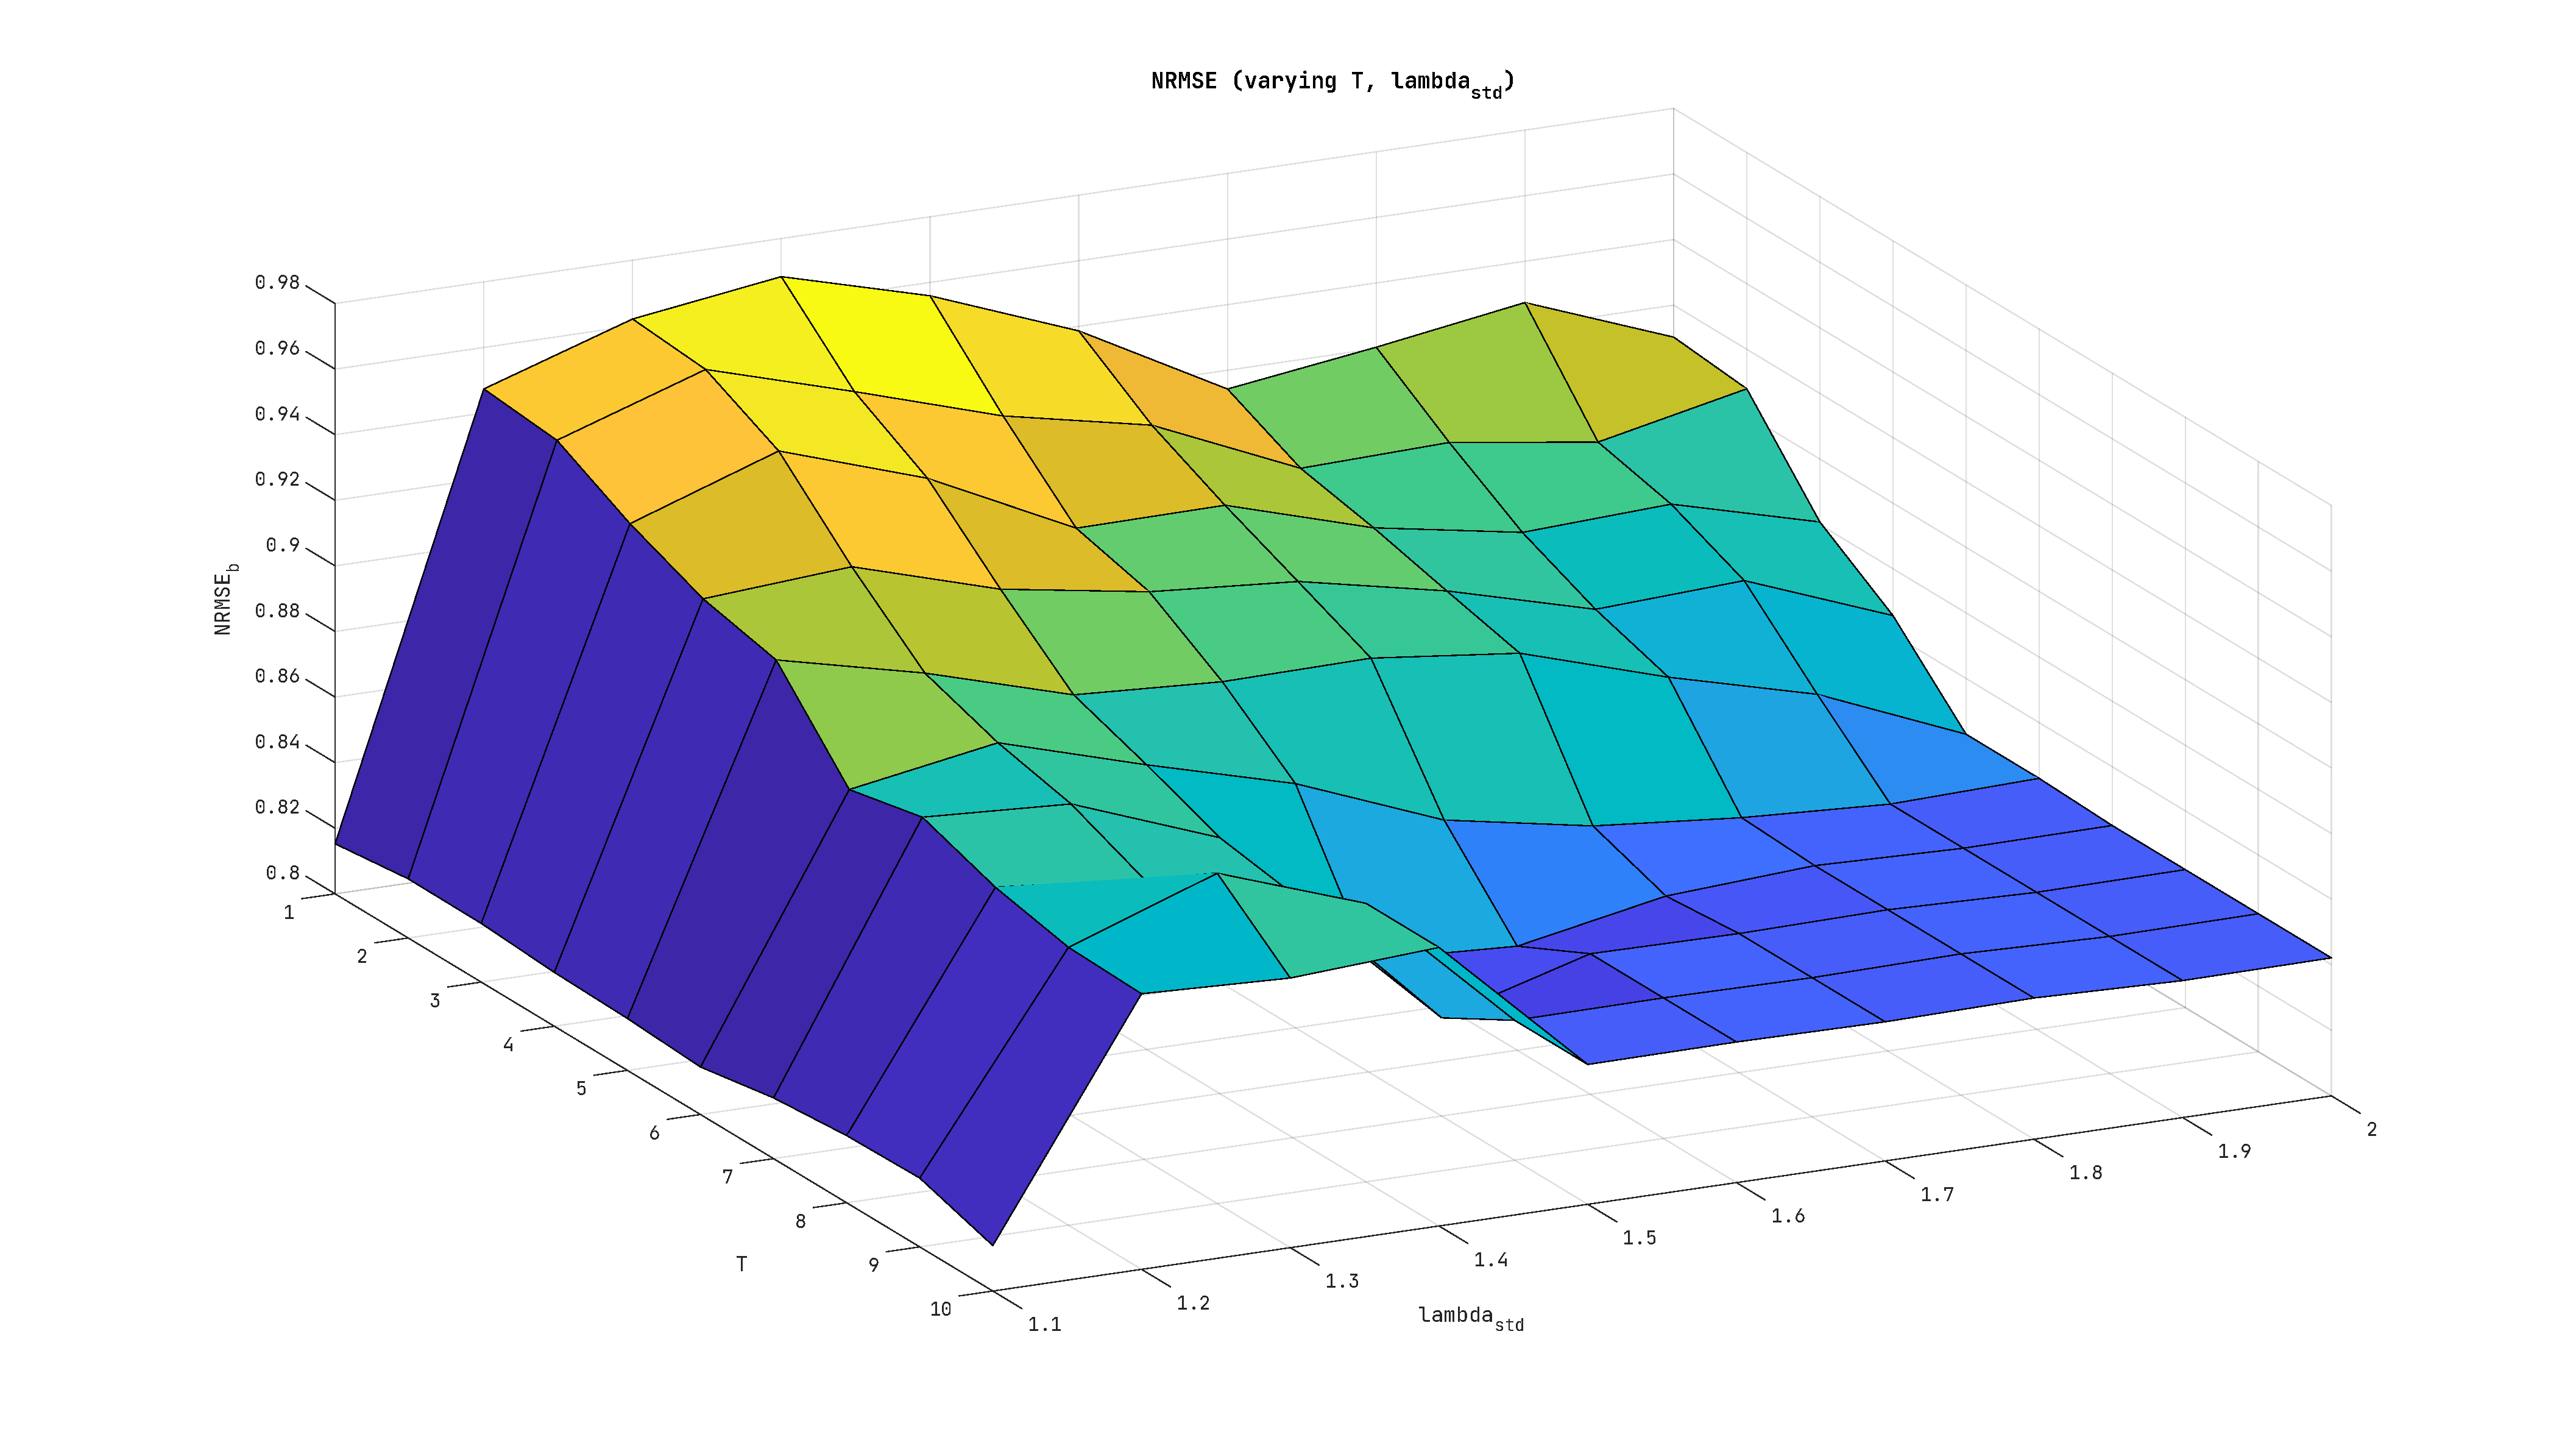
\includegraphics[width=\textwidth]{plots/nrmse_b.svg.pdf}
        \caption{\tl{NRMSE} προβλέψεων κατά τον υπολογισμό των σημείων αλλαγής (\tl{MCPs}), για κάθε τιμή του πλέγματος αναζήτησης ως πρός τον ορίζοντα πρόβλεψης, $T$, και το $\lambda_{std}$ του ορίου απόφασης, $\alpha$}
        \label{fig:nrmse_b}
    \end{center}
\end{figure}

\par Γενικότερα, αναζητούμε τα \textquote{γόνατα} στις αντίστοιχες τρισδιάστατες καμπύλες έτσι ώστε περαιτέρω μεταβολές των αντίστοιχων παραμέτρων να μην είναι πλέον επικερδείς.

\par Επικεντρώνοντας στο πρώτο διάγραμμα και δεδομένου ότι θέλουμε ο αριθμός των \tl{MCPs} να μήν είναι πολύ μεγάλος ή πολύ μικρός, θα επιλέγαμε τις ακόλουθες τιμές (προσεγγιστικά):
\begin{align}
    T \in [5,8] \ \ \ \& \ \ \ \lambda_{std} \in [1.2, 1.5]
    \label{eq:t_lambda_mcps_b}
\end{align}

\textbf{Παρατηρούμε δηλαδή σημαντική μεταβολή στο εύρος της παραμέτρου $\lambda_{std}$ στη χρονοσειρά \tl{B} σε σύγκριση με το αντίστοιχο διάγραμμα της \tl{A}, το οποίο προκύπτει από την απότομη πτώση του διαγράμματος παραπάνω το οποίο με τη σειρά του πιθανότητα οφείλεται στην ύπαρξη μεγάλύτερης τυπικής αποκλίσης στη στάσιχμη χρονοσειρά $X_{b_{deseasoned}}$.}

\par Επικεντρώνοντας τώρα στο διάγραμμα των \tl{NRMSEs} και δεδομένου ότι θέλουμε το \tl{NRMSE} να είναι κατά το δυνατό μικρό, θα επιλέγαμε τις ακόλουθες τιμές (προσεγγιστικά):
\begin{align}
    T \geq 5 \ \ \ \& \ \ \ \lambda_{std} \geq 1.5
    \label{eq:t_lambda_nrmses_b}
\end{align}

\par Συνδυάζοντας τις σχέσεις (\ref{eq:t_lambda_mcps_b}) και (\ref{eq:t_lambda_nrmses_b}) παραπάνω καταλήγουμε ότι οι \tl{hyperparameters} που θα χρησιμοποιηθούν για την εφαρμογή της μεθόδου αυτόματης εύρεσης χρονικών σημείων αλλαγής θα είναι:
\textbf{T = 5 βήματα} και \textbf{λ\textsubscript{\tl{std}} = 1.5}. Οι αντίστοιχες τιμές του \tl{grid search} είναι: \textbf{$\vert$\tl{MCP}$\vert$ = 8 \tl{MCPs}} και \textbf{\tl{NRMSE} = 0.8921}.


\section{Εφαρμογή με Βέλτιστες Παραμέτρους}

Χρησιμοποιώντας τις επιλεγμένες τιμές για τις \tl{hyperparameters} της μεθόδου, δηλαδή ορίζοντα πρόβλεψης έως και 5 βημάτων εμπρός, $T=5$, και παράμετρο ορίου απόφασης στο 1.5, $\lambda_{std}=1.5$, θα τρέξουμε την παραπάνω μέθοδο στη στάσιμη χρονοσειρά που προέκυψε από το βήμα \ref{ch:step3}, $\{X_{b_{deseasoned}}(t)\}$, και στο $ARMA(4,4)$ μοντέλο που προσαρμόστηκε σε αυτή (σχέση \ref{eq:xb_deseasoned_4_4_model}). Παρακάτω, φαίνονται τα σημεία αλλαγής που προκύπτουν από την εκτέλεση της μεθόδους με τις παραπάνω παραμέτρους για κάθε μια από τις επιλογές αναπροσαρμογής του μοντέλου (\textquote{\tl{a}}, \textquote{\tl{b}} ή \textquote{\tl{c}}).

\subsection{Αναπροσαρμογή όταν βρεθεί σημείο αλλαγής}

\textit{Επιλογή \textquote{\tl{c}}}

\begin{figure}[H]
    \begin{center}
        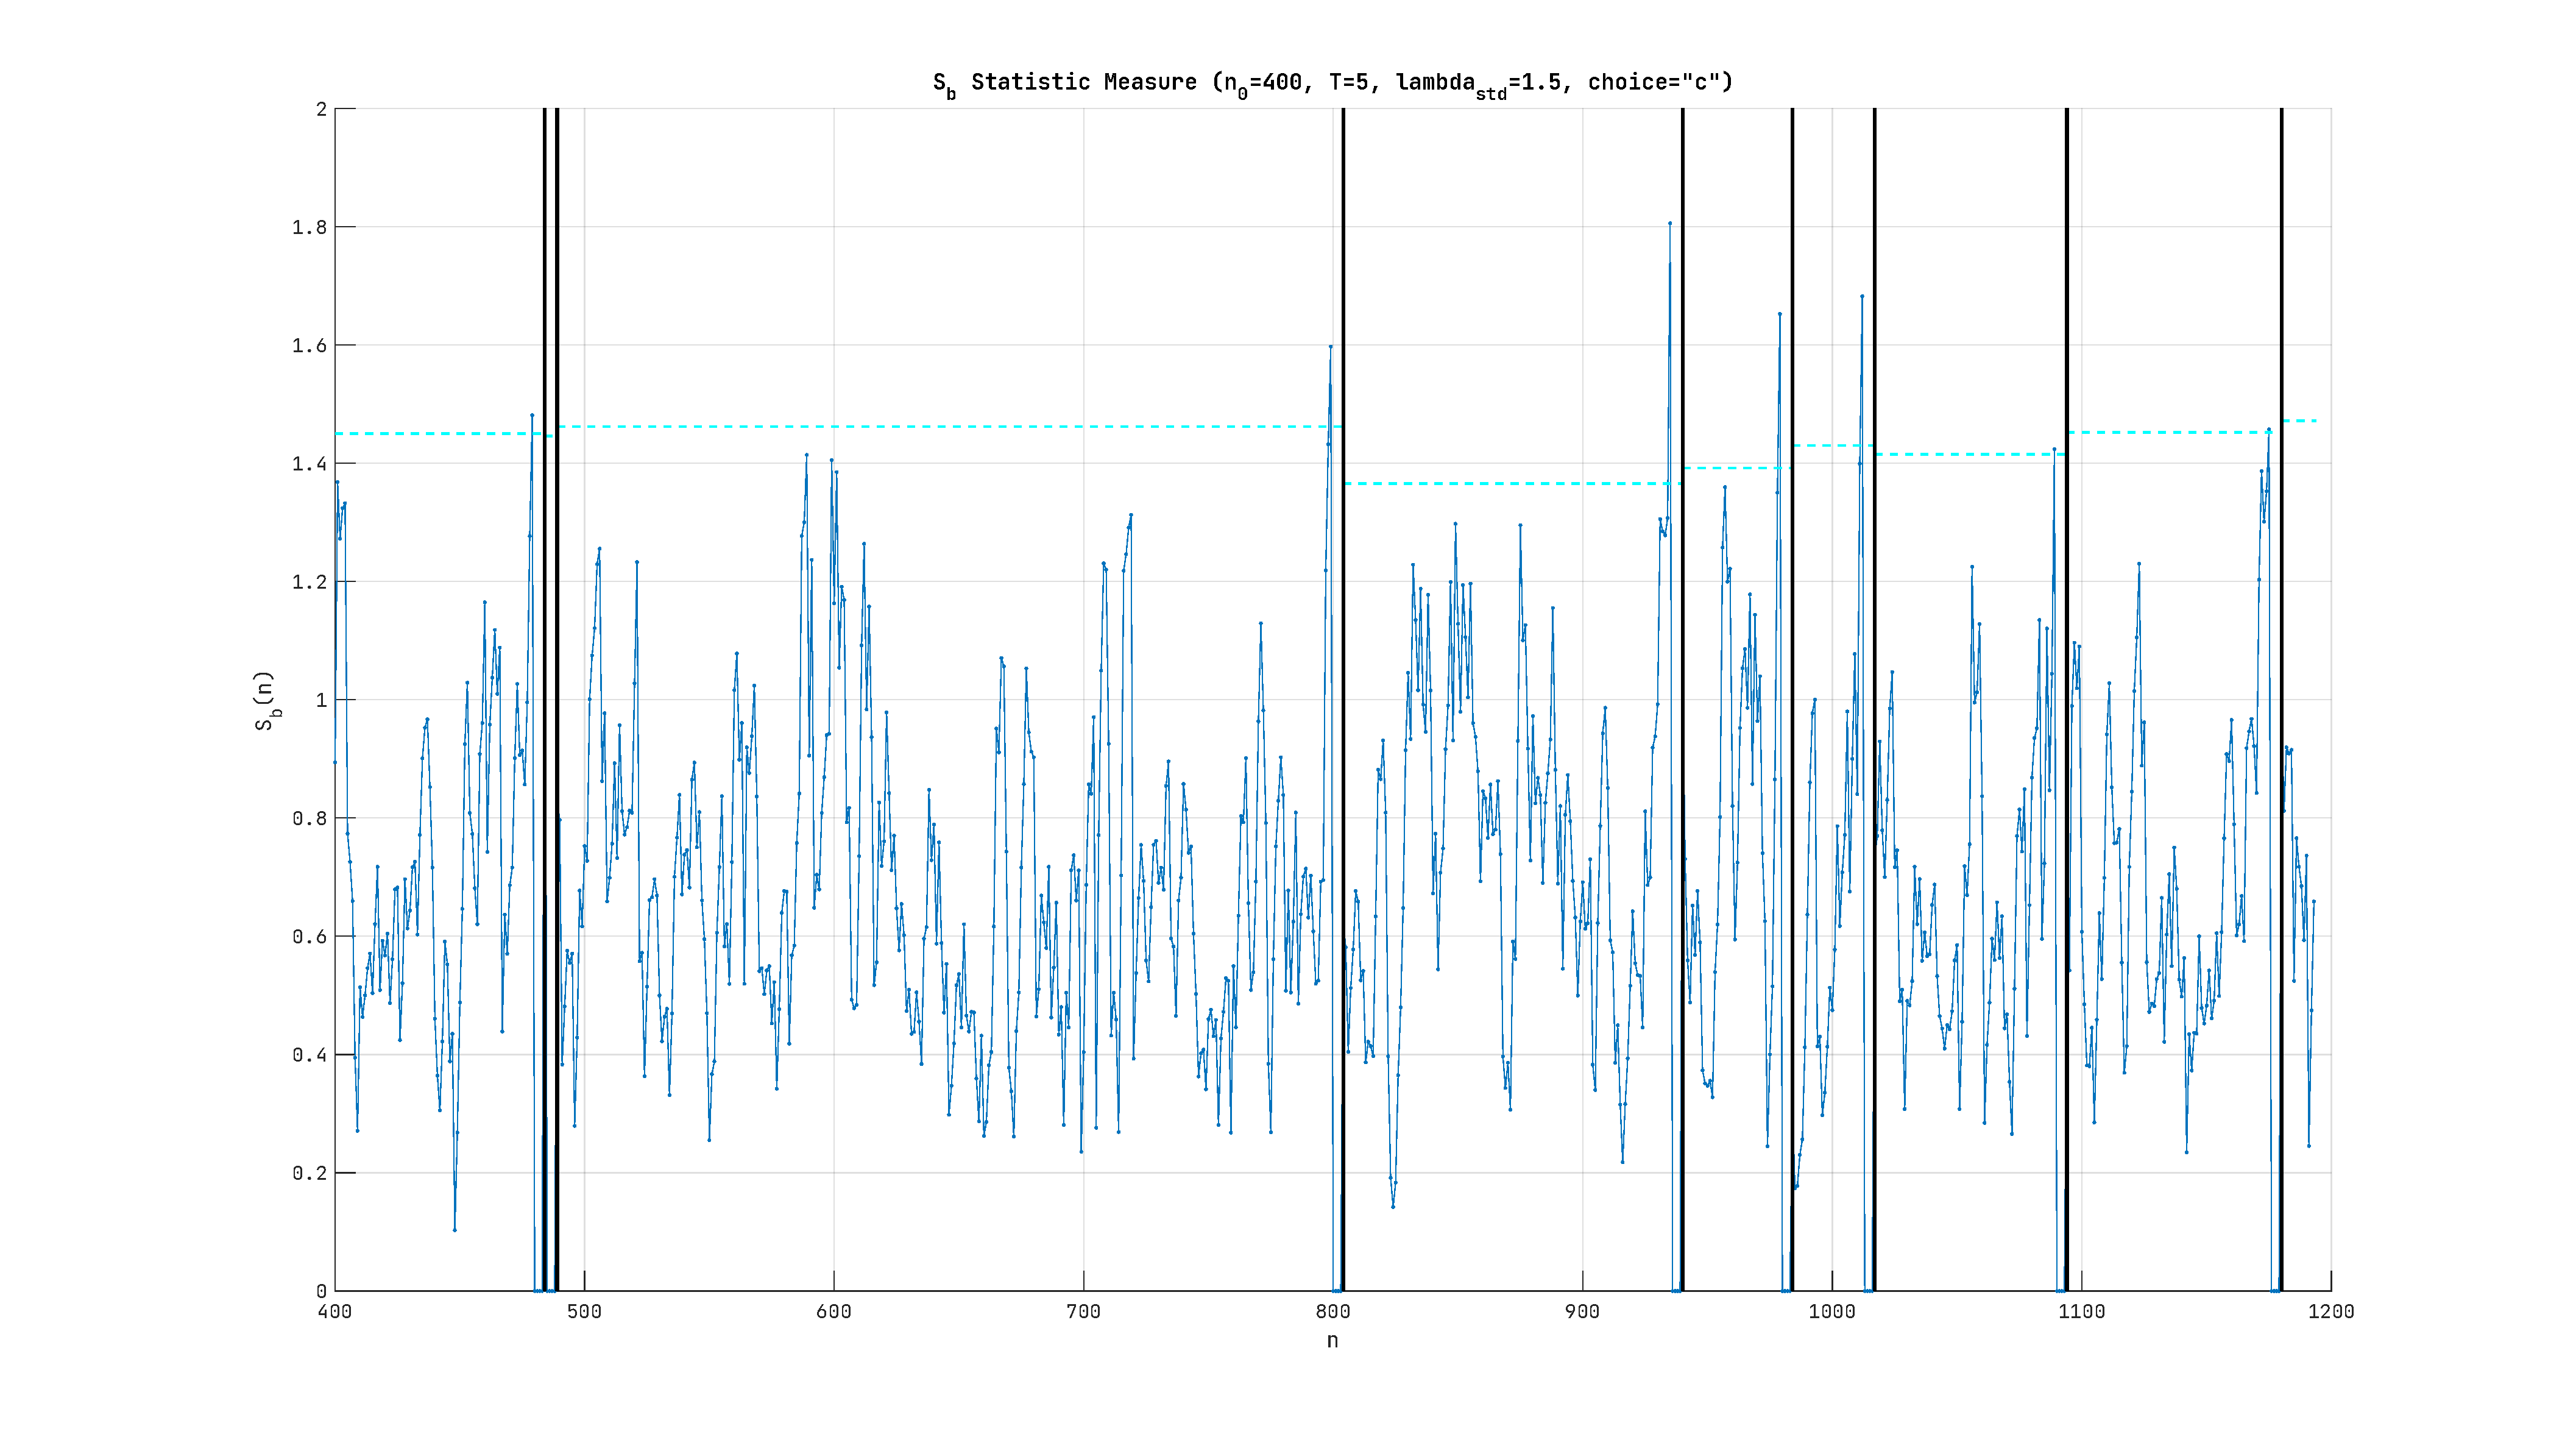
\includegraphics[width=\textwidth]{plots/mcps_xb_opt_c.svg.pdf}
        \caption{Τιμές στατιστικού $S_n$ για έως και 6 βήματα μπροστά πρόβλεψη με $ARMA(4,4)$ της στάσιμης χρονοσειράς $\{X_{b_{deseasoned}}(t)\}$ και για επιλογή αναπροσαρμογής \textquote{\tl{c}} (αναπροσαρμογή όταν βρεθεί σημείο αλλαγής). Σημειώνονται επίσης το κριτήριο απόφασης, $\alpha=1.5*s_x$, (\tl{cyan}) και φυσικά τα σημεία αλλαγής με έντονες κάθετες γραμμές στα εκάστοτε σημεία $n+T$ (μαύρο) - [\tl{NRMSE}=0.892, \ 76.2\tl{sec}]}
        \label{fig:mcps_xb_opt_c}
    \end{center}
\end{figure}

Παρακάτω, τα ίδια σημεία αλλαγής απεικονίζονται στην αρχική χρονοσειρά προβολών του βίντεο \tl{B}:

\begin{figure}[H]
    \begin{center}
        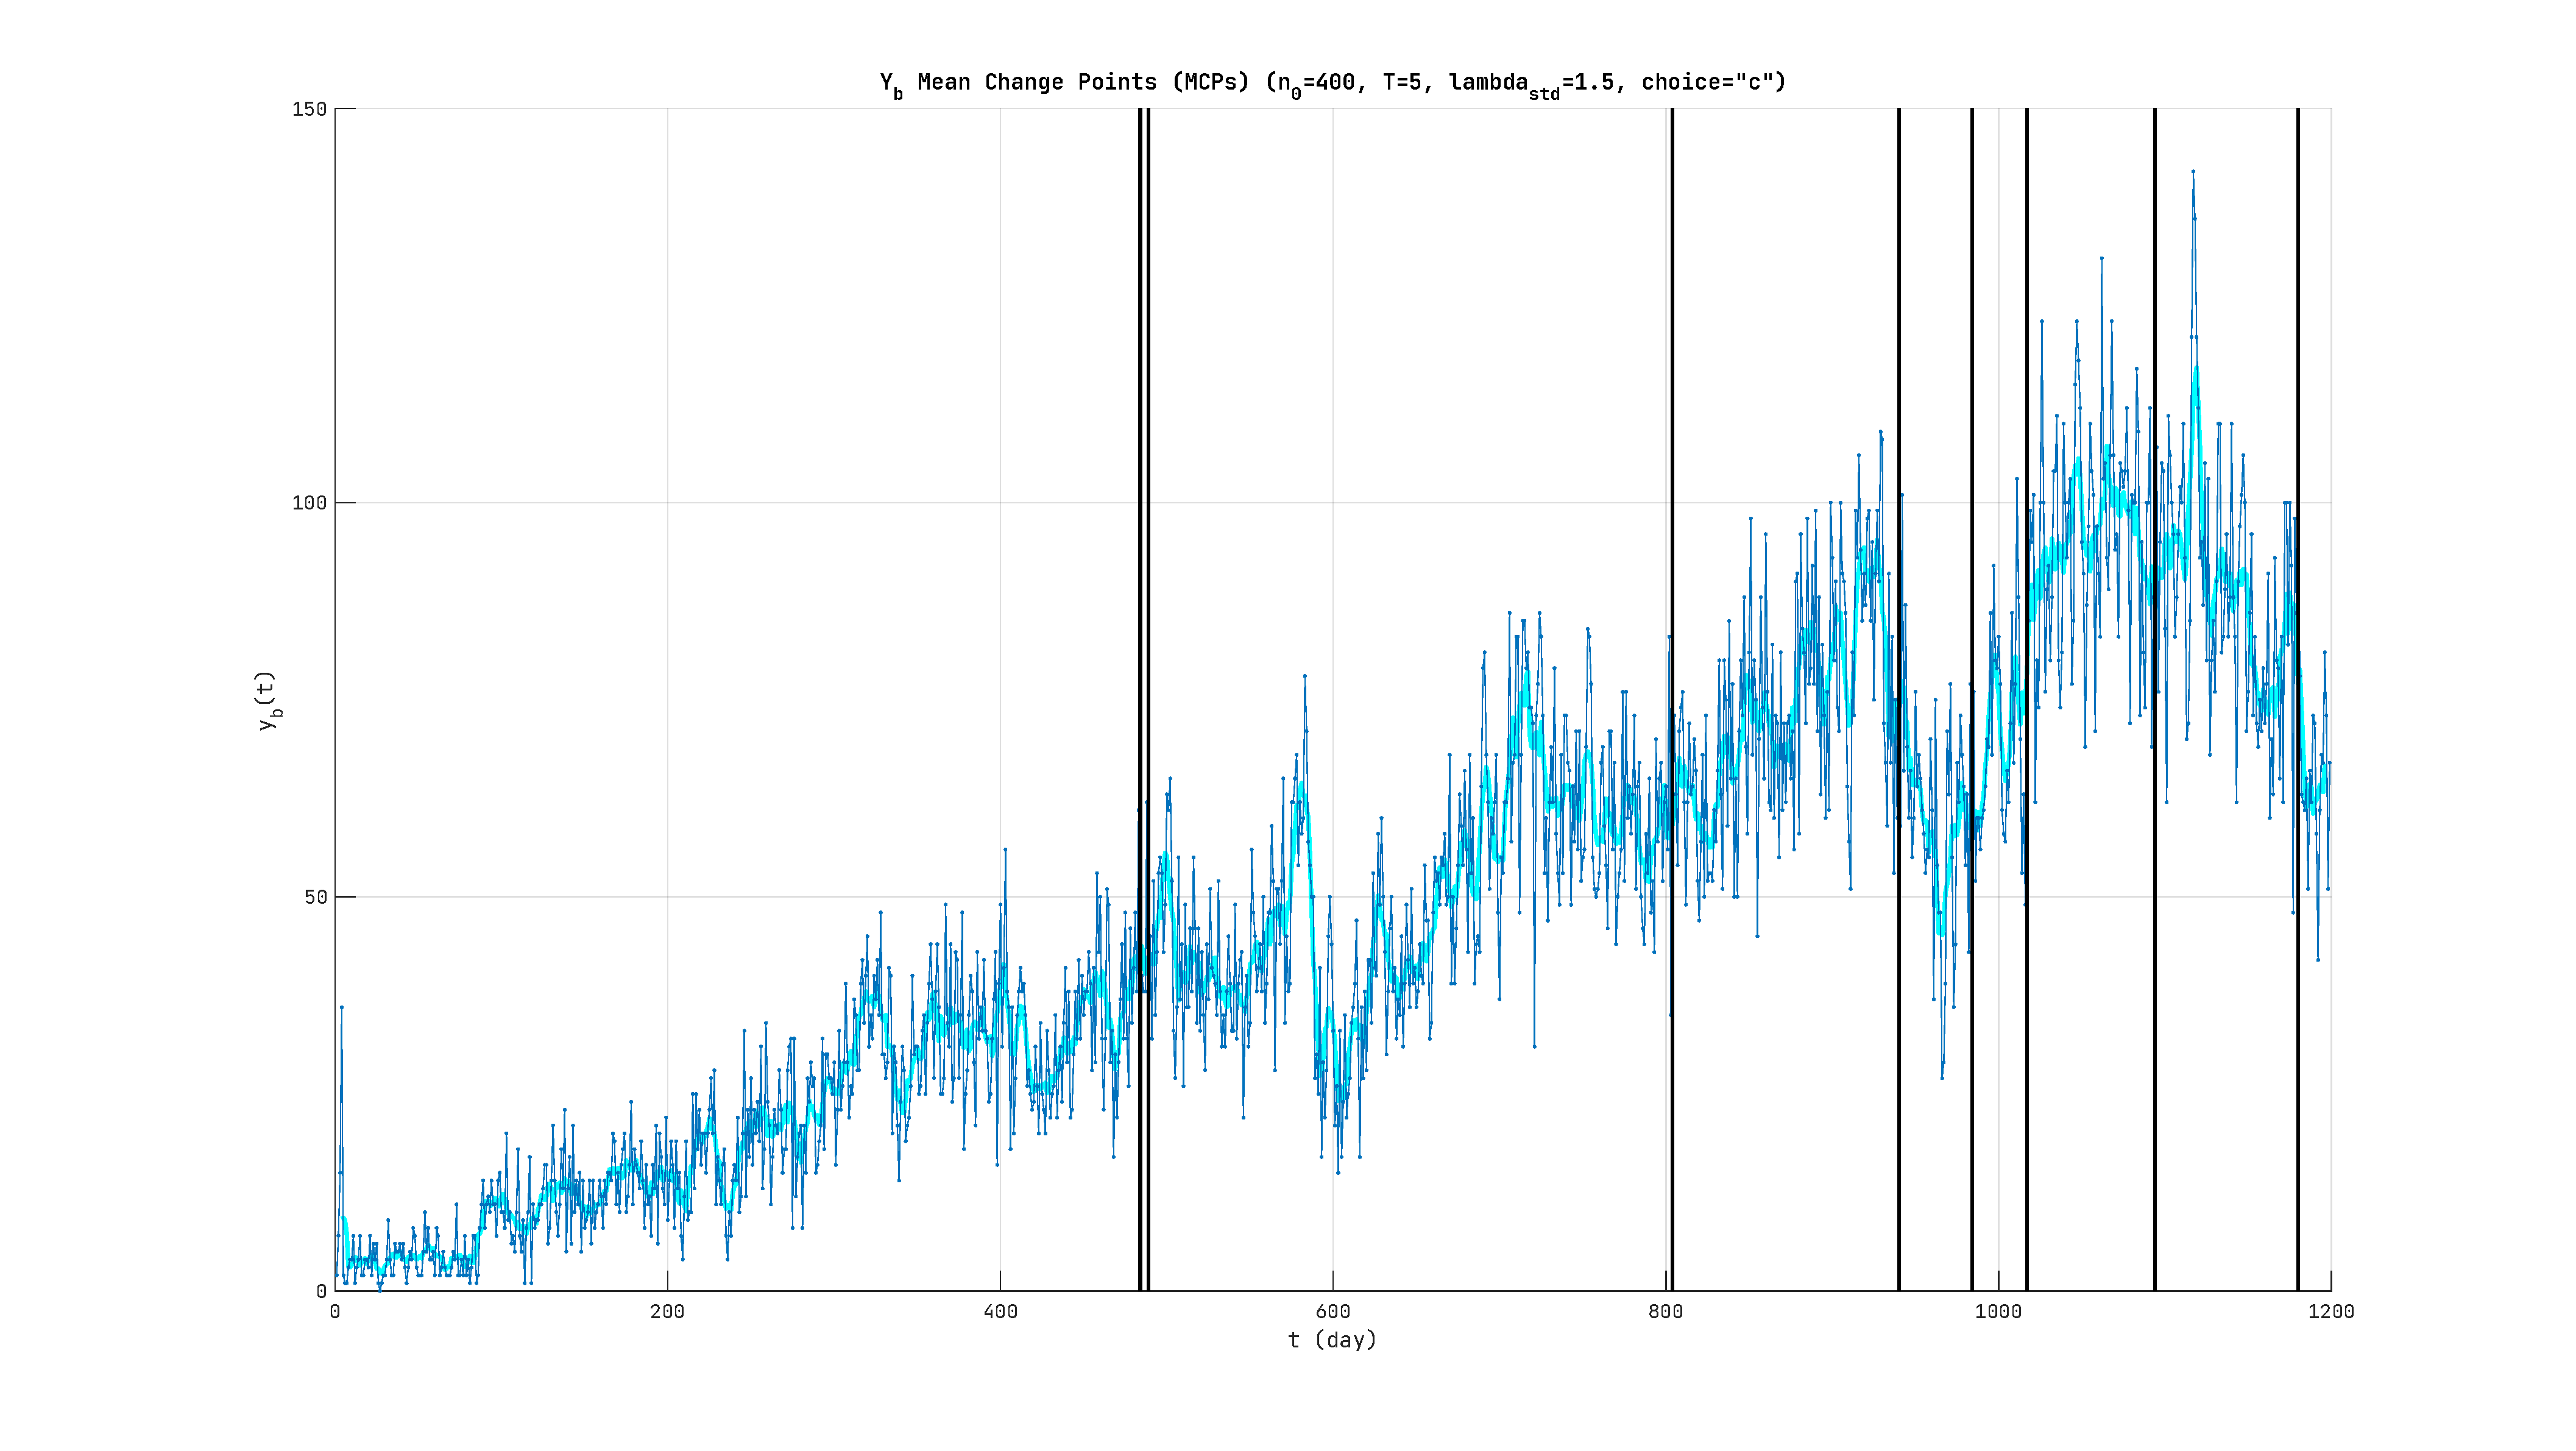
\includegraphics[width=\textwidth]{plots/mcps_yb_opt_c.svg.pdf}
        \caption{Διάγραμμα ιστορίας της αρχικής χρονοσειράς $\{Y_b(t)\}$ (μπλε) μαζί με τα σημεία αλλαγής (μαύρο) που επιλέχθηκαν από την ανάλυση της στάσιμης εκδοχής της με τις βέλτιστες παραμέτρους, καθώς και εκτίμηση της τάσης με φίλτρο κινούμενου μέσου τάξης 7 ($MA(7)$ \tl{smoothing}) - επιλογή \textquote{\tl{c}}}
        \label{fig:mcps_yb_opt_c}
    \end{center}
\end{figure}


\subsection{Αναπροσαρμογή σε κάθε χρονική στιγμή}

\textit{Επιλογή \textquote{\tl{b}}}

\par Τα ίδια διαγράμματα παρουσιάζονται για την επιλογή αναπροσαρμογής \textquote{\tl{b}} (αναπροσαρμογή σε κάθε χρονική στιγμή) ενώ ακολουθεί σύντομος σχολιασμός:

\begin{figure}[H]
    \begin{center}
        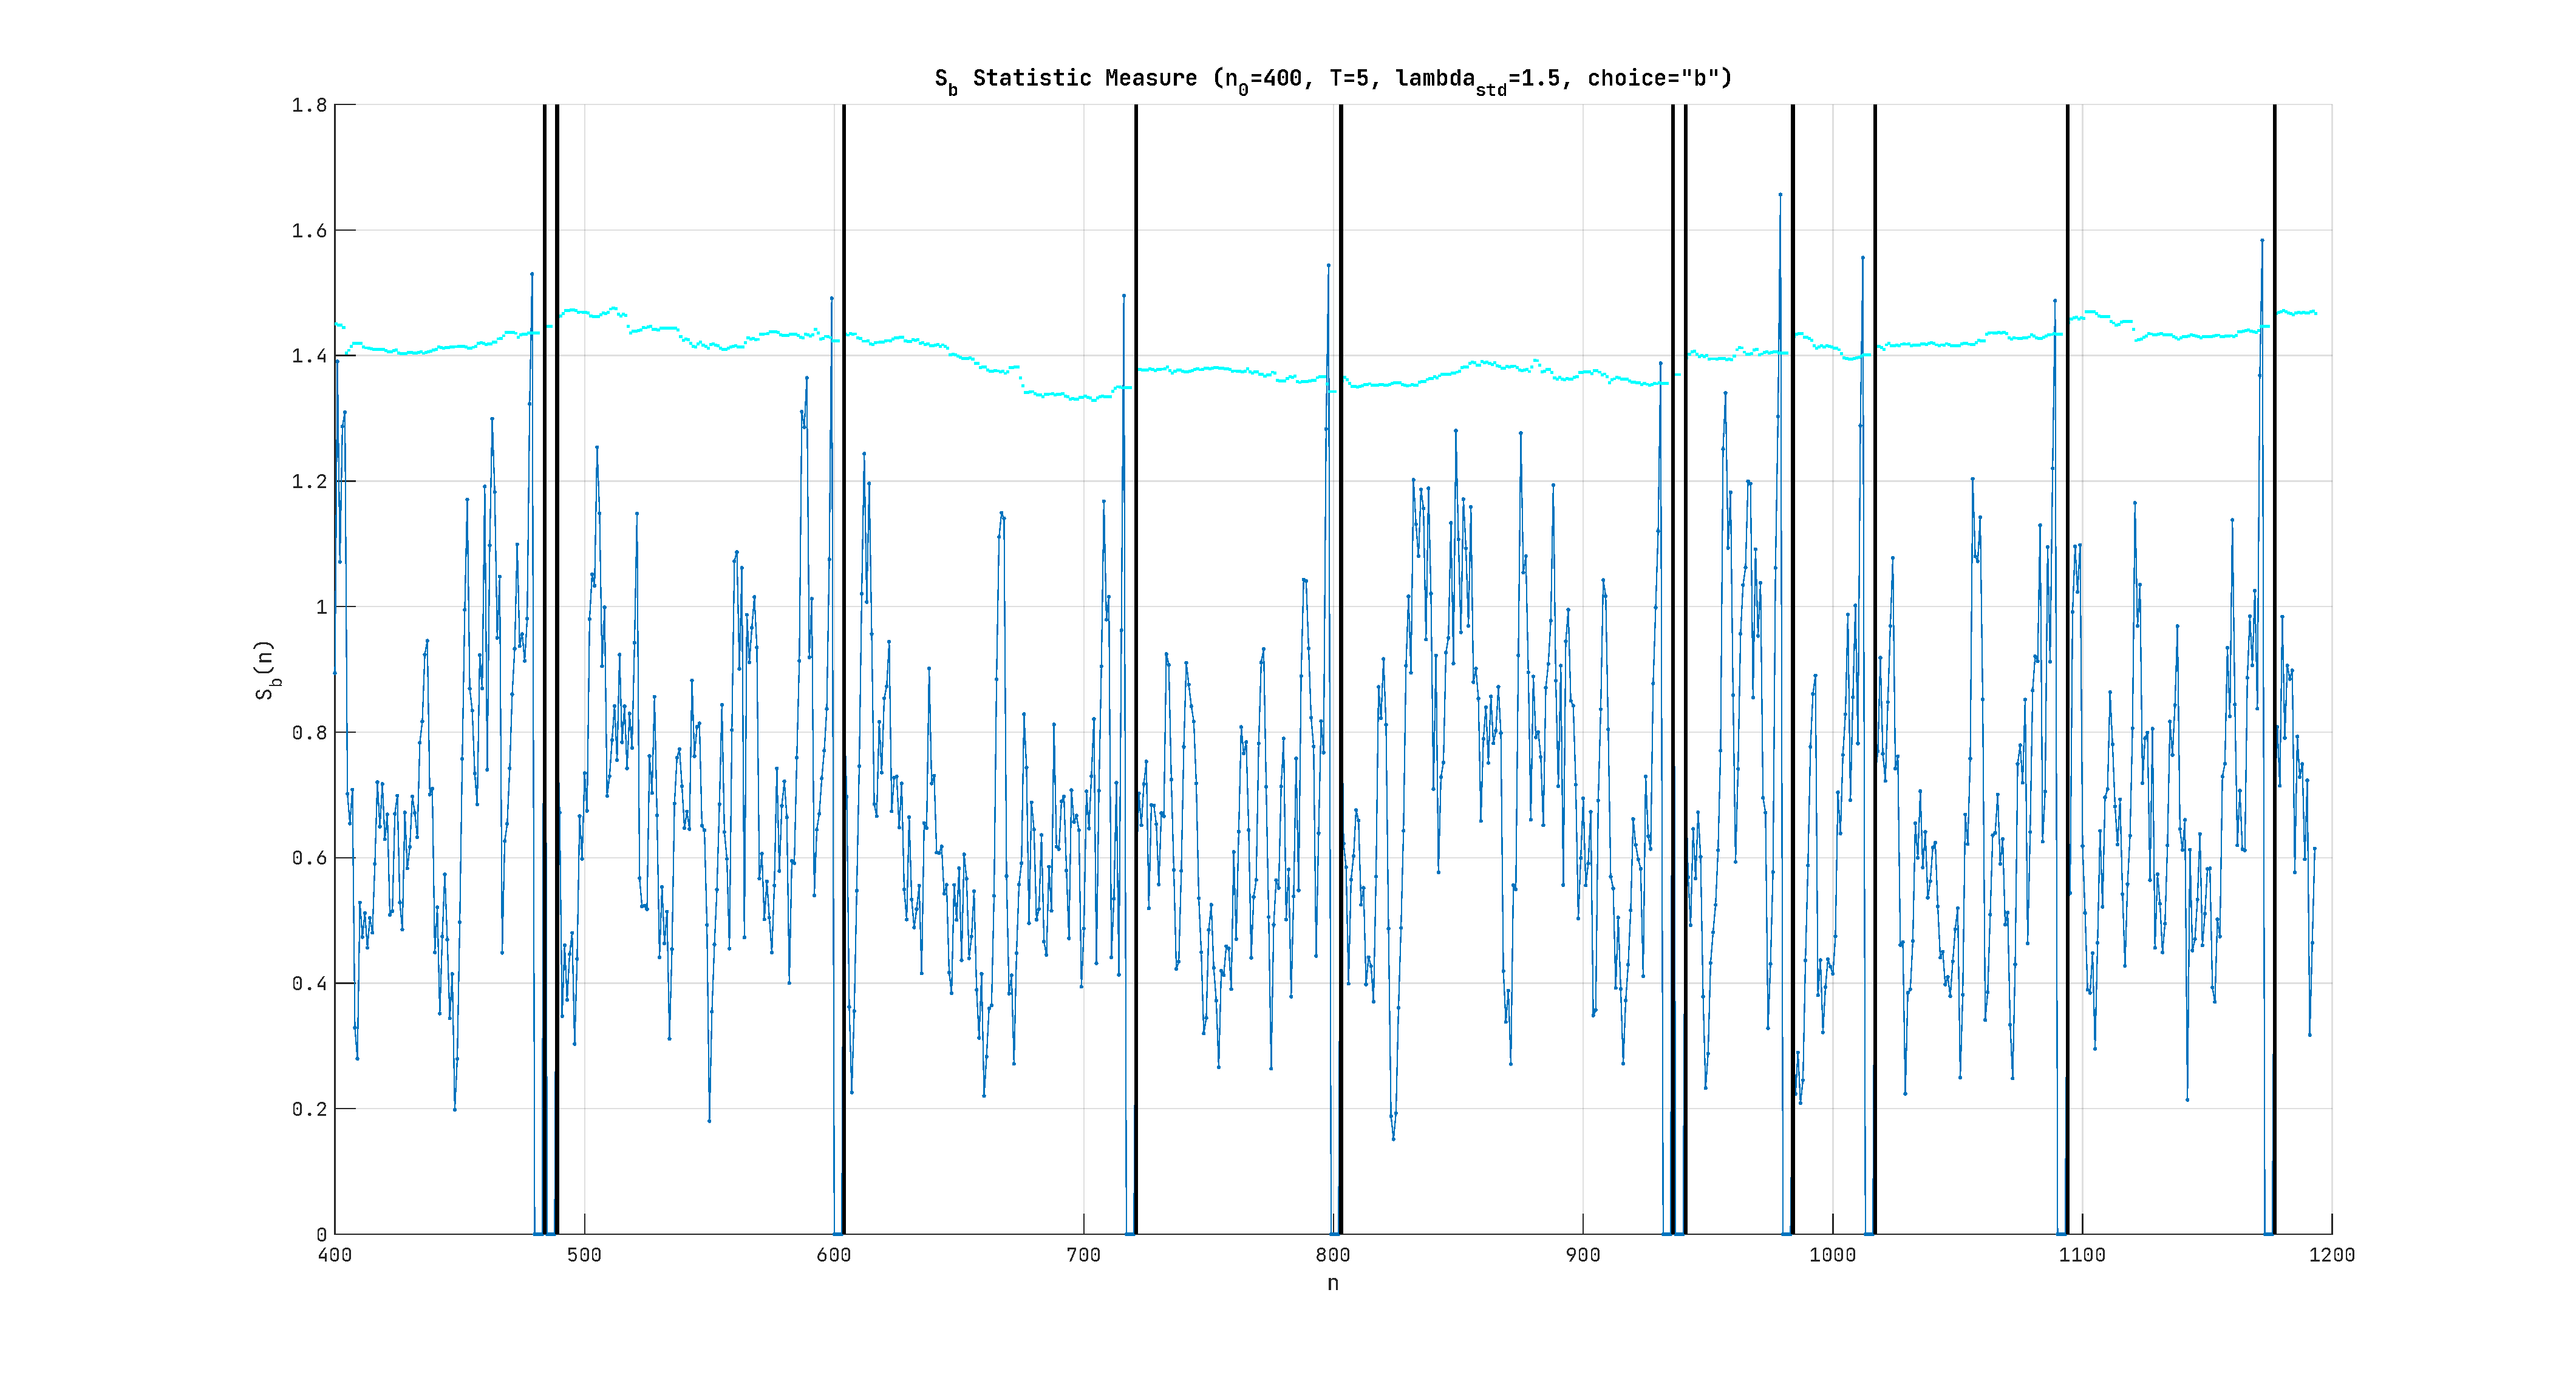
\includegraphics[width=\textwidth]{plots/mcps_xb_opt_b.svg.pdf}
        \caption{Τιμές στατιστικού $S_n$ για έως και 5 βήματα μπροστά πρόβλεψη με $ARMA(4,4)$ της στάσιμης χρονοσειράς $\{X_{b_{deseasoned}}(t)\}$ και για επιλογή αναπροσαρμογής \textquote{\tl{b}} (αναπροσαρμογή σε κάθε χρονική στιγμή). Σημειώνονται επίσης το κριτήριο απόφασης, $\alpha=1.5*s_x$, (\tl{cyan}) και φυσικά τα σημεία αλλαγής με έντονες κάθετες γραμμές στα εκάστοτε σημεία $n+T$ (μαύρο) - [\tl{NRMSE}=0.893, \ 244.1\tl{sec}]}
        \label{fig:mcps_xb_opt_b}
    \end{center}
\end{figure}

Παρακάτω, τα ίδια σημεία αλλαγής απεικονίζονται στην αρχική χρονοσειρά προβολών του βίντεο \tl{B}:

\begin{figure}[H]
    \begin{center}
        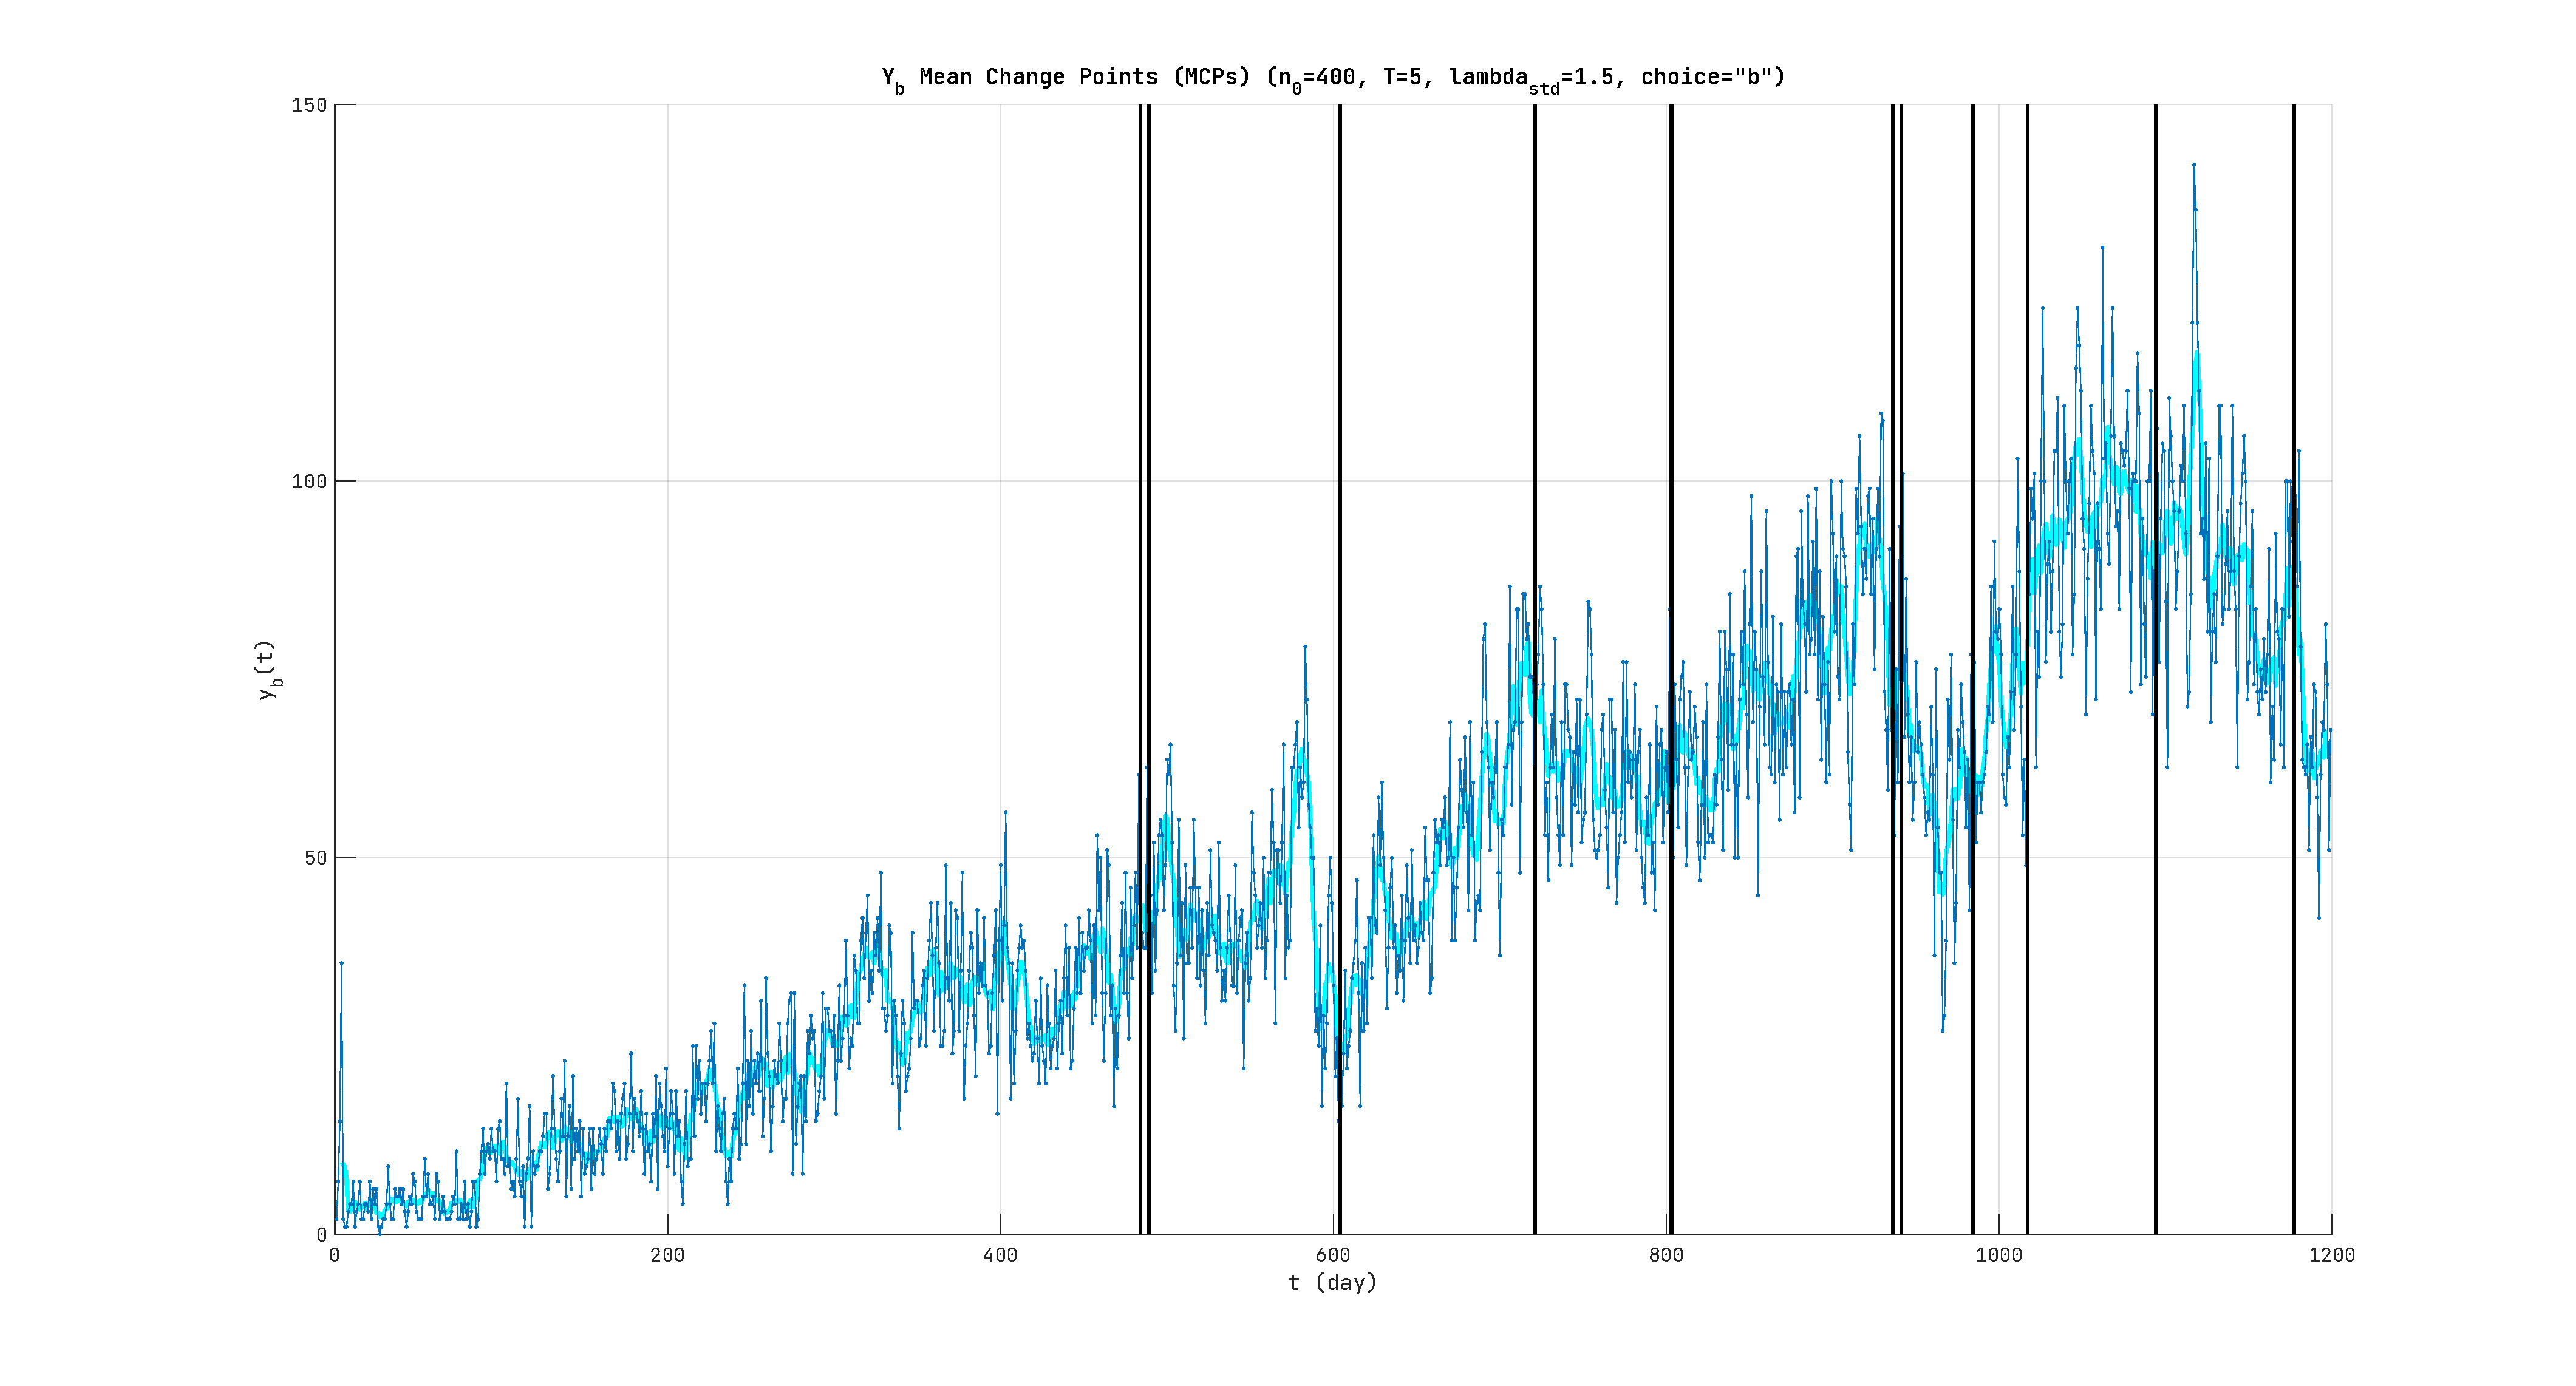
\includegraphics[width=\textwidth]{plots/mcps_yb_opt_b.svg.pdf}
        \caption{Διάγραμμα ιστορίας της αρχικής χρονοσειράς $\{Y_b(t)\}$ (μπλε) μαζί με τα σημεία αλλαγής (μαύρο) που επιλέχθηκαν από την ανάλυση της στάσιμης εκδοχής της με τις βέλτιστες παραμέτρους, καθώς και εκτίμηση της τάσης με φίλτρο κινούμενου μέσου τάξης 7 ($MA(7)$ \tl{smoothing}) - επιλογή \textquote{\tl{b}}}
        \label{fig:mcps_yb_opt_b}
    \end{center}
\end{figure}

Βλέποντας τα τελευταία δύο (2) διαγράμματα και συγκρίνοντάς τα με αυτά της επιλογής \textquote{\tl{c}} κάνουμε τις εξής παρατηρήσεις:
\begin{enumerate}
    \item Τα σημεία αλλαγής είναι περισσότερα σε αριθμό (11 πλέον \tl{vs.} 6 με την επιλογή \textquote{\tl{c}}) έχοντας σημεία στις ίδιες θέσεις αλλά προσθέτοντας και επιπλέον σημεία αλλαγής. Αυτό είναι αποτέλεσμα αφενός της κυμάτωσης που εμφανίζεται πλέον στο όριο απόφασης αλλά κυρίως στο ότι πλέον τα σφάλματα $S_n$ εμφανίζουν περισσότερες \textquote{κορυφές}.
    \item Το όριο απόφασης (\tl{cyan} διακεκομμένη γραμμή) φαίνεται να έχει πολύ μεγαλύτερη διακύμανση σε σύγκριση με αυτό της επιλογής \textquote{\tl{c}}, κάτι απολύτως αναμενόμενο αφού η αναπροσαρμογή γίνεται πλέον σε κάθε βήμα / χρονική στιγμή και άρα αντίστοιχα η δειγματική τυπική απόκλιση των παρατηρήσεων του \tl{training set} αλλάζει συνεχώς
\end{enumerate}

\subsection{Χωρίς Αναπροσαρμογή}

\textit{Επιλογή \textquote{\tl{a}}}

\par Τέλος, τα ίδια διαγράμματα παρουσιάζονται για την επιλογή αναπροσαρμογής \textquote{\tl{a}} (καμία αναπροσαρμογή - διατήρηση του μοντέλου που προσαρμόστηκε στις πρώτες 400 παρατηρήσεις της στάσιμης χρονοσειράς), ενώ ακολουθεί σύντομος σχολιασμός:

\begin{figure}[H]
    \begin{center}
        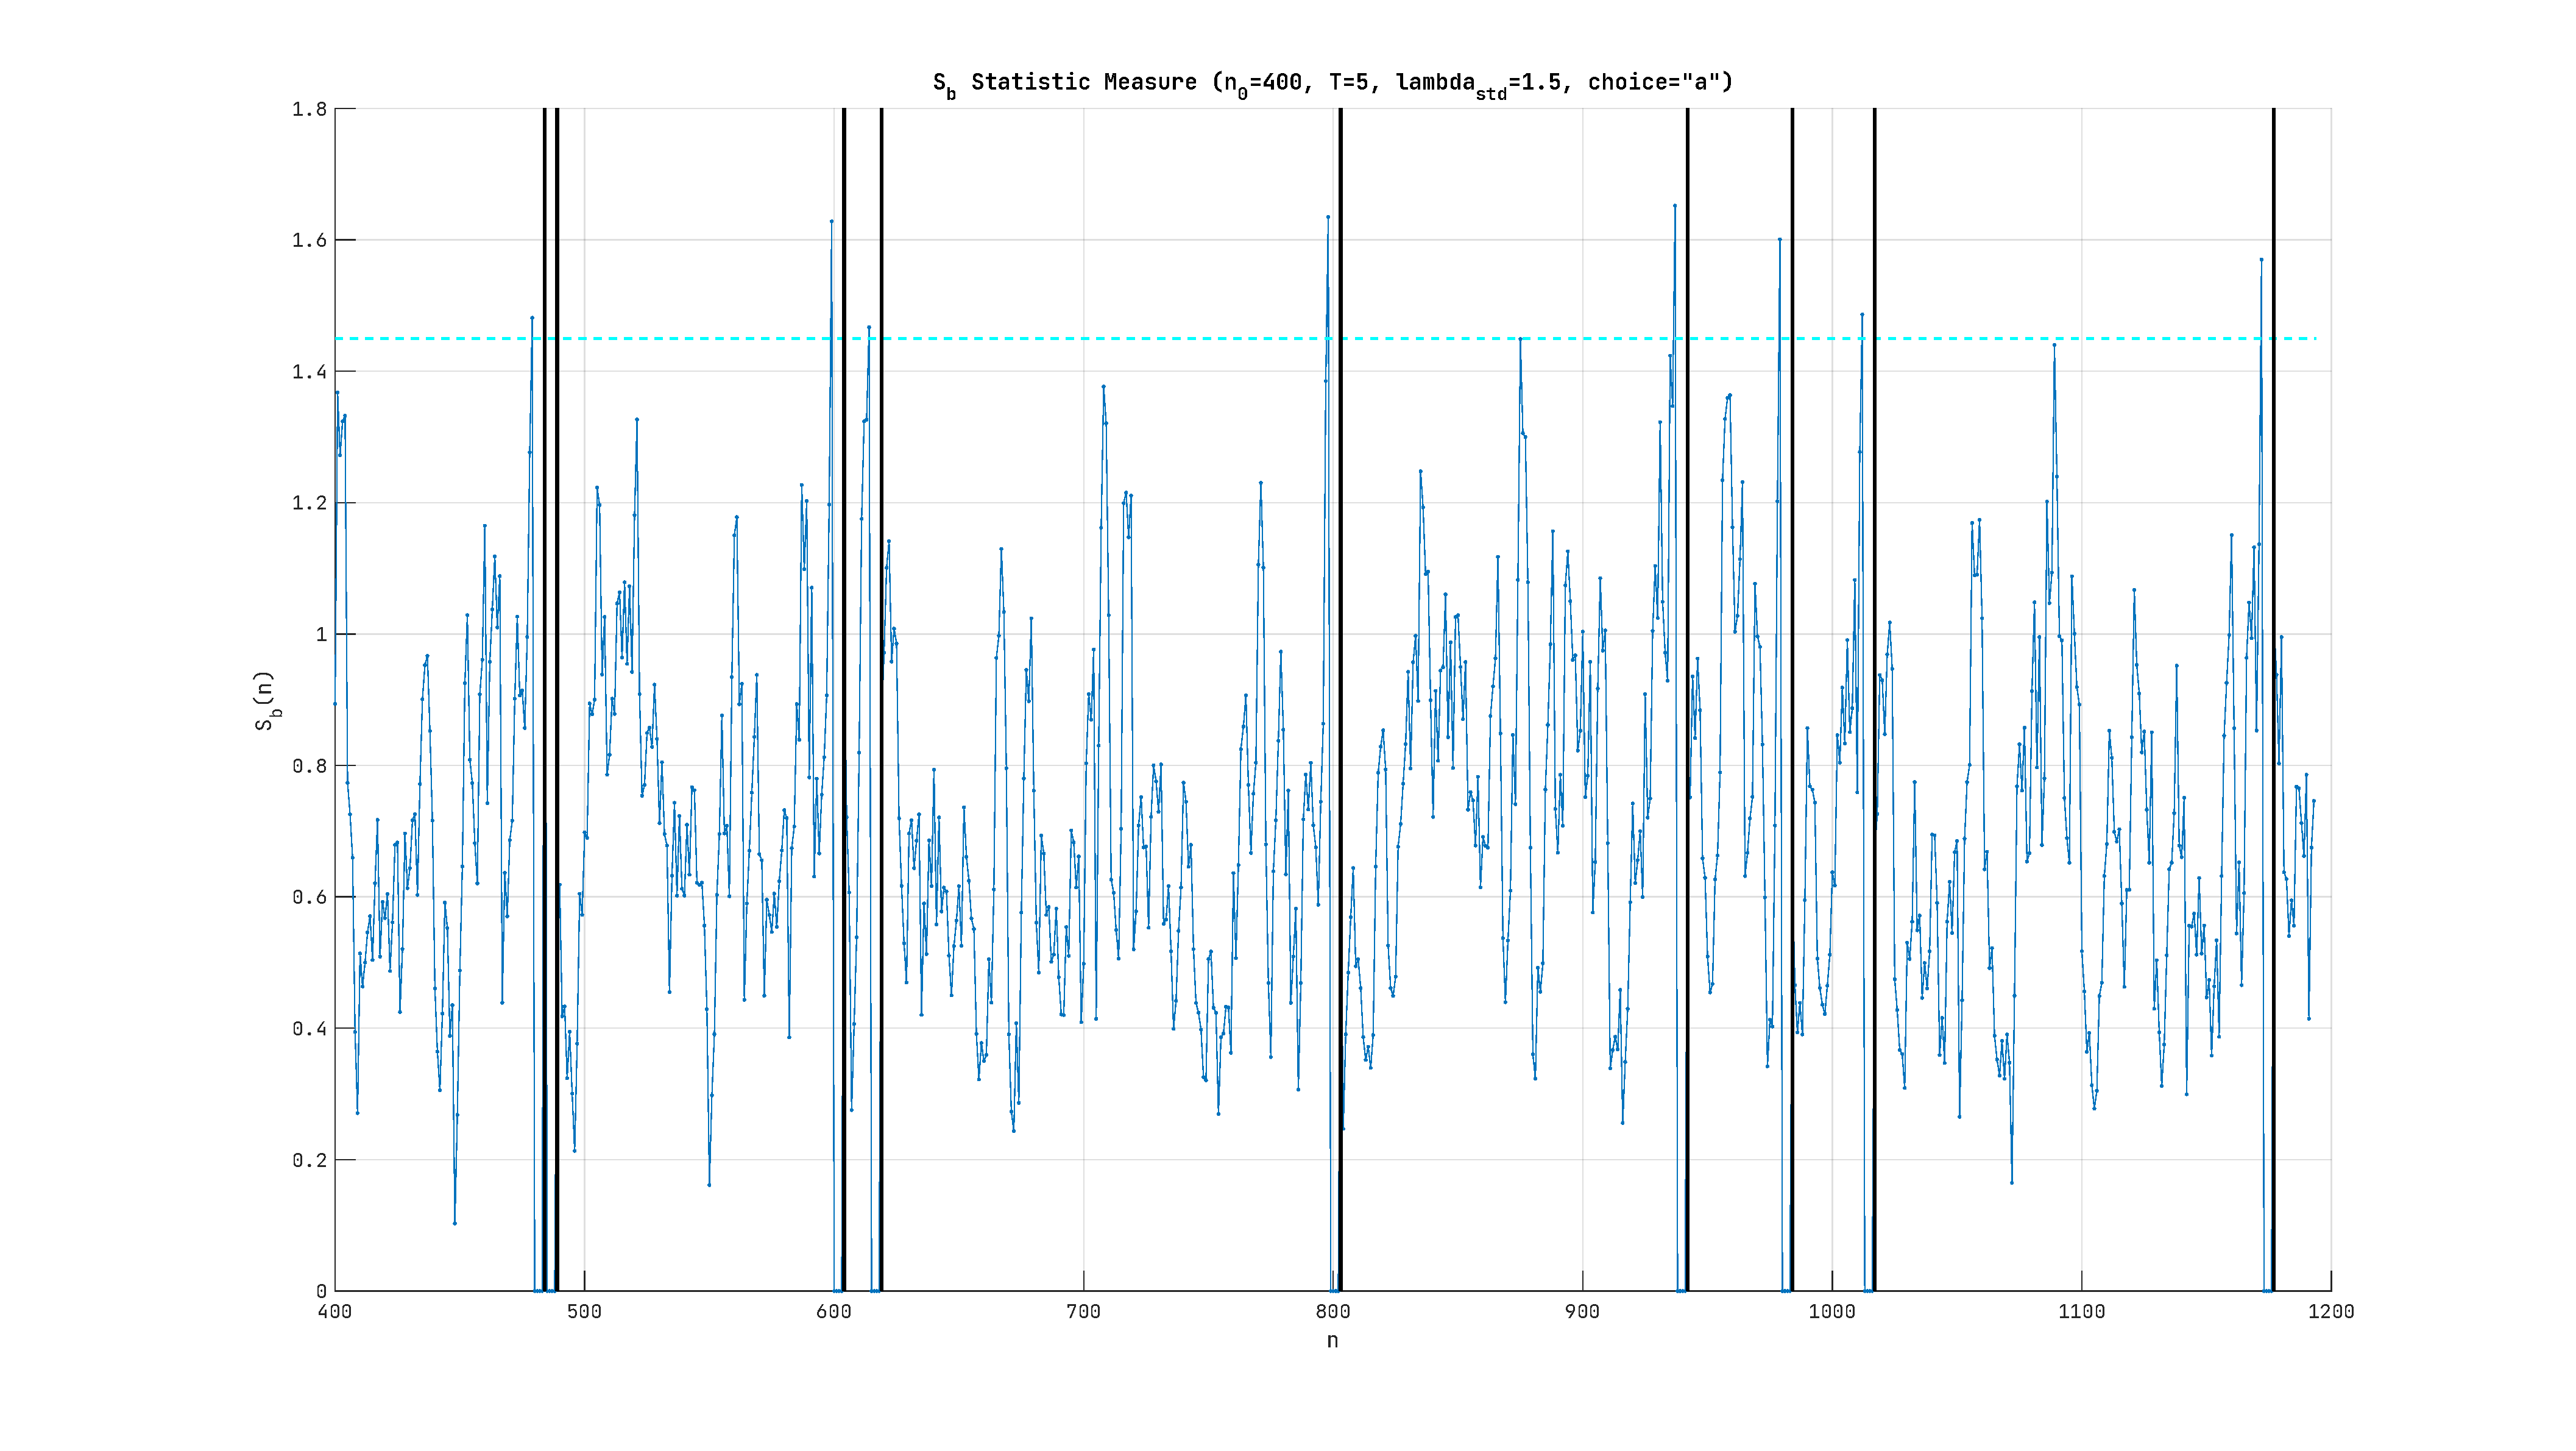
\includegraphics[width=\textwidth]{plots/mcps_xb_opt_a.svg.pdf}
        \caption{Τιμές στατιστικού $S_n$ για έως και 5 βήματα μπροστά πρόβλεψη με $ARMA(4,4)$ της στάσιμης χρονοσειράς $\{X_{b_{deseasoned}}(t)\}$ και για επιλογή αναπροσαρμογής \textquote{\tl{a}} (χωρίς αναπροσαρμογή). Σημειώνονται επίσης το κριτήριο απόφασης, $\alpha=1.5*s_x$, (\tl{cyan}) και φυσικά τα σημεία αλλαγής με έντονες κάθετες γραμμές στα εκάστοτε σημεία $n+T$ (μαύρο) - [\tl{NRMSE}=0.899, \ 61.1\tl{sec}]}
        \label{fig:mcps_xb_opt_a}
    \end{center}
\end{figure}

Παρακάτω, τα ίδια σημεία αλλαγής απεικονίζονται στην αρχική χρονοσειρά προβολών του βίντεο \tl{B}:

\begin{figure}[H]
    \begin{center}
        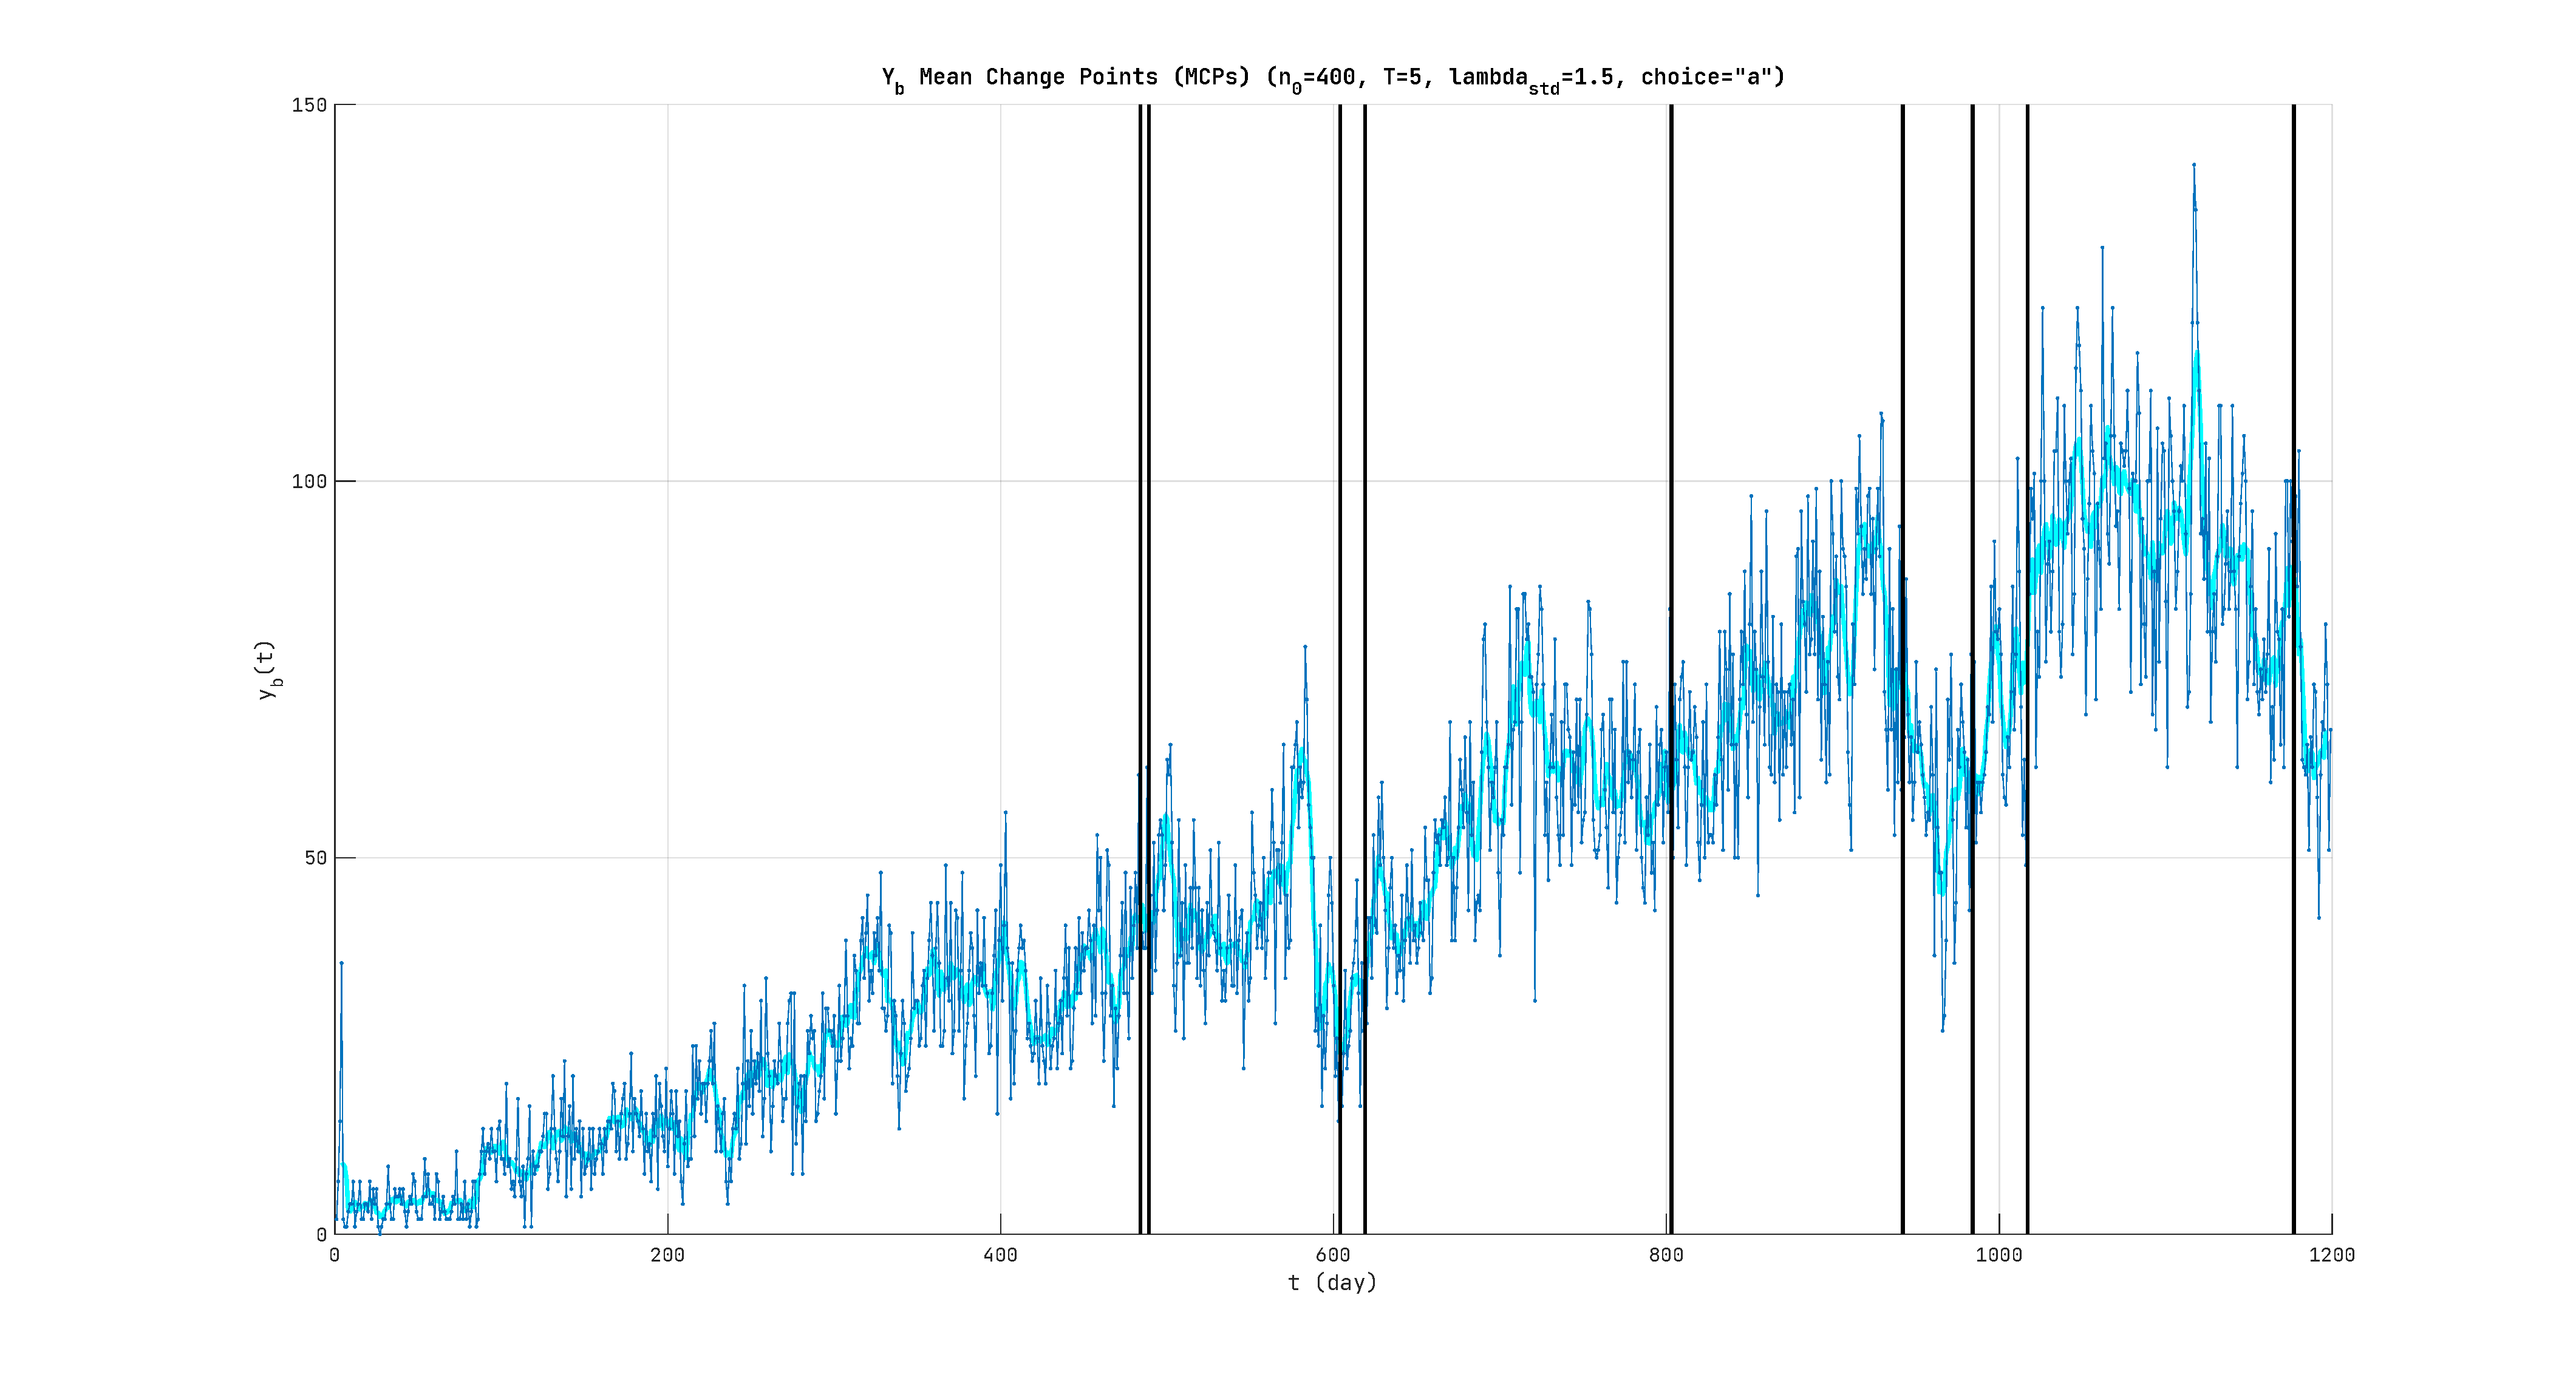
\includegraphics[width=\textwidth]{plots/mcps_yb_opt_a.svg.pdf}
        \caption{Διάγραμμα ιστορίας της αρχικής χρονοσειράς $\{Y_b(t)\}$ (μπλε) μαζί με τα σημεία αλλαγής (μαύρο) που επιλέχθηκαν από την ανάλυση της στάσιμης εκδοχής της με τις βέλτιστες παραμέτρους, καθώς και εκτίμηση της τάσης με φίλτρο κινούμενου μέσου τάξης 7 ($MA(7)$ \tl{smoothing}) - επιλογή \textquote{\tl{a}}}
        \label{fig:mcps_yb_opt_a}
    \end{center}
\end{figure}

Βλέποντας τα τελευταία δύο (2) διαγράμματα και συγκρίνοντάς τα με αυτά της επιλογής \textquote{\tl{c}} κάνουμε τις εξής παρατηρήσεις:
\begin{enumerate}
    \item Τα σημεία αλλαγής είναι και εδώ περισσότερα κατά 1 (9 \tl{vs.} 8) αλλά και σε διαφορετικές θέσεις τα 4 από τα 9. Παρόλα αυτά, τα σημεία της επιλογής \textquote{\tl{b}} οδηγούν σε χαμηλότερο NRMSE.
    \item Το όριο απόφασης (\tl{cyan} διακεκομμένη γραμμή), όπως αναφέρθηκε, παραμένει συνεχώς σταθερό, κάτι πιθανότατα μη επιθυμητό
\end{enumerate}

Καταληκτικά, η πιο κατάλληλη επιλογή για αναπροσαρμογή του μοντέλου πρόβλεψης είναι η επιλογή \textquote{\tl{c}} (αναπροσαρμογή όταν βρεθεί σημείο αλλαγής) καθώς συνδυάζει καλή υπολογιστική συμπεριφορά αλλά ταυτόχρονα επιτυγχάνει και το μικρότερο \tl{NRMSE} των προβλέψεων κατά την εκτέλεση της μεθόδου. Πρέπει να σημειωθεί επίσης ότι αυτή η επιλογή χρησιμοποιήθηκε και κατά το \tl{grid search} των \tl{hyperparameters} (σχήματα \ref{fig:mcps_count_b} και \ref{fig:nrmse_b} παραπάνω).

\subsection{Συμπερασματικά Σχόλια}

Συμπερασματικά και επιγραμματικά, είναι σκόπιμο να αναφερθεί ότι η προσέγγιση εξαγωγής σημείων αλλαγής με την μέθοδο που αναλύθηκε στα βήματα 4-5 παραπάνω, \textbf{θα μπορούσε να χρησιμοποιηθεί για αυτόματο εντοπισμό αυτών των σημείων}. Συγκεκριμένα, με την υπόθεση ότι το $T$ (ορίζοντας πρόβλεψης) και το $\lambda_{std}$ έχουν κατάλληλα επιλεγεί ενώ το μοντέλο αναπροσαρμόζεται κάθε φορά που βρίσκεται ένα σημείο αλλαγής, τότε αυτή η μέθοδος φαίνεται να επιτυγχάνει την εύρεση σημείων αλλαγής τα οποία - τουλάχιστον οπτικά - φαίνονται να βρίσκονται σε περιοχές που όντως η ζήτηση παρουσιάζει βραχεία έξαρση ή βύθιση.